%%%% main.tex, 2022/08/10, 2.5
%%%% Copyright (C) 2020 Vinicius Pegorini (vinicius@utfpr.edu.br)
%%
%% This work may be distributed and/or modified under the conditions of the
%% LaTeX Project Public License, either version 1.3 of this license or (at your
%% option) any later version.
%% The latest version of this license is in
%%   http://www.latex-project.org/lppl.txt
%% and version 1.3 or later is part of all distributions of LaTeX version
%% 2005/12/01 or later.
%%
%% This work has the LPPL maintenance status `maintained'.
%%
%% The Current Maintainer of this work is Vinicius Pegorini.
%%
%% This work consists of the files utfprpb.cls, utfprpb.tex, and
%% utfprpb-dados.tex.
%%
%% The Current Maintainer of this work is Vinicius Pegorini.
%% Updated by:
%% - Marco Aurélio Graciotto Silva;
%% - Rogério Aparecido Gonçalves;
%% - Luiz Arthur Feitosa dos Santos.
%%
%% This work consists of the files utfpr.cls, main.tex, and
%% variaveis.tex.
%% A brief description of this work is in readme.md.

%% ####################################################
%%
%% >> Atenção - Leia isso antes de usar esse template<< 
%%
%% Esse template foi desenvolvido por professores,  com a intenção de ajudar os alunos com as entregas na biblioteca. Não há uma equipe especializada e dedicada mantendo tal template, mas sim professores trabalhando além das suas funções básicas, que são: ensino, pesquisa e extensão.
%
%% Também os mantenedores deste template não são especializados em LaTeX, muito menos em normas da ABNT. Todos que contribuíram com o template fizeram isso visando deixá-lo o mais próximo possível das normas da ABNT e das regras, anseios e expectativas da biblioteca da UTFPR. É muito importante entender que os desenvolvedores do template não têm relação direta com a biblioteca ou com a ABNT. Ou seja, não são os desenvolvedores do template que ditam as regras e normas dos textos que devem ser entregues à biblioteca.

%%É válido informar também, que como não há uma equipe dedicada e especializada, o tempo para colaborar com o template é curto. Desta forma, pode ser que não sejam empregadas as melhores técnicas, métodos e ferramentas para o desenvolvimento do template. Também pode acontecer do template não atender completamente todos os anseios e exigências da ABNT e da biblioteca, pois por exemplo, muitas regras de redação possuem questões interpretativas. Assim, o template sempre estará em contínua evolução e seria extremamente interessante que as pessoas (alunos,  professores,  técnicos e entusiastas) colaborarem com a evolução do template. Toda ajuda será bem vinda! Isso pode ser feito enviando e-mail para os desenvolvedores, desta forma, assim que possível esses vão tentar melhorar o template.

%%O template é apenas mais uma ferramenta para o desenvolvimento de trabalhos para a biblioteca. Todavia, podem existir outros templates LaTeX. Assim como há templates em outros formatos, que não o LaTeX. O mais importante é que qualquer pessoa, utilizando a princípio qualquer ferramenta, pode desenvolver textos que atendem os requisitos da biblioteca apenas estudando, interpretando e seguindo as regras da UTFPR e da ABNT, que estão disponíveis na página Web da instituição. O template é só um facilitador.

%%Por fim,  é necessário entender que infelizmente o ambiente LaTeX pode ser complexo e gerar resultados distintos dependendo do: sistema operacional,  pacotes LaTeX utilizados,  configurações alteradas, editor utilizado, a forma que está sendo redigida textos, figuras,  etc. Assim não há como garantir que o resultado final será o esperado.  Dito tudo isso,  >>UTILIZE ESSE TEMPLATE POR SUA CONTA E RISCO<<. Os desenvolvedores e colaboradores deste template não se responsabilizam pelo resultado do uso deste template e se eximem de qualquer responsabilidade.

%###################################################


% Luiz - pdfa: inclusão do pdfa
\PassOptionsToPackage{
	pdfa
}{hyperref}

%% Classe e opções de documento
\documentclass[%% Opções
%% -- Opções da classe memoir --
  12pt,%% Tamanho da fonte: 10pt, 11pt, 12pt, etc.
  a4paper,%% Tamanho do papel: a4paper (A4), letterpaper (carta), etc.
  % fleqn,%% Alinhamento das equações à esquerda (comente para alinhamento centralizado)
  % leqno,%% Numeração das equações no lado esquerdo (comente para lado direito)
  oneside,%% Impressão dos elementos textuais e pós-textuais: oneside (anverso) ou twoside (anverso e verso, se mais de 100 p.)
  openright,%% Impressão da primeira página dos capítulos: openright (anverso), openleft (verso) ou openany (anverso e verso)
%% -- Opções da classe abntex2 --
  sumario = abnt-6027-2012,%% Formatação do sumário: tradicional (estilo tradicional) ou abnt-6027-2012 (norma ABNT 6027-2012)
  chapter = TITLE,%% Títulos de capítulos em maiúsculas (comente para desabilitar)
  % luiz - comentar section para ser minusculo
  %section = TITLE,%% Títulos de seções secundárias em maiúsculas (comente para desabilitar)
  % subsection = TITLE,%% Títulos de seções terciárias em maiúsculas (comente para desabilitar)
  % subsubsection = TITLE,%% Títulos de seções quartenárias em maiúsculas (comente para desabilitar),
%% -- Opções da classe utfprpgtex --
  pretextualoneside,%% Impressão dos elementos pré  -textuais: pretextualoneside (anverso) ou pretextualtwoside (anverso e verso)
  fontetimes,%% Fonte do texto: fontetimes (times), fontearial (arial) ou fontecourier (courier)
  % vinculoscoloridos,%% Cores nos vínculos (citações, arquivos, links, url, etc.) (comente para desabilitar)
  semrecuonosumario,%% Remoção do recuo dos itens no sumário (comente para adição do recuo, se estilo tradicional)
  usemakeindex,%% Compilação de glossários e índices utilizando makeindex (comente para desabilitar)
  % legendascentralizadas,%% Alinhamento das legendas centralizado (comente para alinhamento à esquerda)
  %aprovacaoestiloppg,%% Folha de aprovação do programa de pós-graduação no estilo do PPG (comente para estilo padrão)
  pardeassinaturas,%% Assinaturas na folha de aprovação em até duas colunas (comente para em uma única coluna)
  % linhasdeassinaturas,%% Linhas de assinaturas na folha de aprovação (comente para remover as linhas)
%% -- Opções do pacote babel --
  english,%% Idioma adicional para hifenização
  french,%% Idioma adicional para hifenização
  spanish,%% Idioma adicional para hifenização
  brazil,%% Idioma principal do documento (último da lista)
]{utfpr}%% Classe utfpr

% Luiz: pdfa: necessário para criar pdfa
\usepackage[a-3b,mathxmp]{pdfx}[2018/12/22] % você pode escolher entre a-1b, a-2b, a-3b - o template ainda não suporta o a-Xa de 

%%%% configuracoes.tex, 2022/05/02, 2.4a

%% ####################################################
%%
%% >> Atenção - Leia isso antes de usar esse template<< 
%%
%% Esse template foi desenvolvido por professores,  com a intenção de ajudar os alunos com as entregas na biblioteca. Não há uma equipe especializada e dedicada mantendo tal template, mas sim professores trabalhando além das suas funções básicas, que são: ensino, pesquisa e extensão.
%
%% Também os mantenedores deste template não são especializados em LaTeX, muito menos em normas da ABNT. Todos que contribuíram com o template fizeram isso visando deixá-lo o mais próximo possível das normas da ABNT e das regras, anseios e expectativas da biblioteca da UTFPR. É muito importante entender que os desenvolvedores do template não têm relação direta com a biblioteca ou com a ABNT. Ou seja, não são os desenvolvedores do template que ditam as regras e normas dos textos que devem ser entregues à biblioteca.

%%É válido informar também, que como não há uma equipe dedicada e especializada, o tempo para colaborar com o template é curto. Desta forma, pode ser que não sejam empregadas as melhores técnicas, métodos e ferramentas para o desenvolvimento do template. Também pode acontecer do template não atender completamente todos os anseios e exigências da ABNT e da biblioteca, pois por exemplo, muitas regras de redação possuem questões interpretativas. Assim, o template sempre estará em contínua evolução e seria extremamente interessante que as pessoas (alunos,  professores,  técnicos e entusiastas) colaborarem com a evolução do template. Toda ajuda será bem vinda! Isso pode ser feito enviando e-mail para os desenvolvedores, desta forma, assim que possível esses vão tentar melhorar o template.

%%O template é apenas mais uma ferramenta para o desenvolvimento de trabalhos para a biblioteca. Todavia, podem existir outros templates LaTeX. Assim como há templates em outros formatos, que não o LaTeX. O mais importante é que qualquer pessoa, utilizando a princípio qualquer ferramenta, pode desenvolver textos que atendem os requisitos da biblioteca apenas estudando, interpretando e seguindo as regras da UTFPR e da ABNT, que estão disponíveis na página Web da instituição. O template é só um facilitador.

%%Por fim,  é necessário entender que infelizmente o ambiente LaTeX pode ser complexo e gerar resultados distintos dependendo do: sistema operacional,  pacotes LaTeX utilizados,  configurações alteradas, editor utilizado, a forma que está sendo redigida textos, figuras,  etc. Assim não há como garantir que o resultado final será o esperado.  Dito tudo isso,  >>UTILIZE ESSE TEMPLATE POR SUA CONTA E RISCO<<. Os desenvolvedores e colaboradores deste template não se responsabilizam pelo resultado do uso deste template e se eximem de qualquer responsabilidade.

%###################################################

%% Pacotes carregados nas classes:
%%   memoir: abstract, appendix, array, booktabs, ccaption, chngcntr, chngpage, dcolumn, delarray, enumerate, epigraph, framed,
%%           ifmtarg, ifpdf, index, makeidx, moreverb, needspace, newfile, nextpage, parskip, patchcmd, setspace, shortvrb, showidx,
%%           tabularx, titleref, titling, tocbibind, tocloft, verbatim, verse.
%%   memoir (similares): crop, fancyhdr, geometry, sidecap, subfigure, titlesec.
%%   abntex2: babel, bookmark, calc, enumitem, ifthen, hyperref, textcase.
%%   utfprpgtex: abntex2cite, ae, algorithmic, amsmath, backref, breakurl, caption, cmap, color, eepic, epic, epsfig, etoolbox,
%%               fancyhdr, fix-cm, fontenc, glossaries, graphics, graphicx, helvet, hyphenat, indentfirst, inputenc, lastpage,
%%               morewrites, nomencl, sfmath, sistyle, substr, times, xtab.


%% Pacotes adicionais (\usepackage[options]{package})
\usepackage{bigdelim, booktabs, colortbl, longtable, multirow}%% Ferramentas para tabelas
\usepackage{amssymb, amstext, amsthm, icomma}%% Ferramentas para linguagem matemática
\usepackage{pifont, textcomp, wasysym}%% Símbolos de texto
\usepackage{lipsum}				% para geração de dummy text
\usepackage{subfig}             % para adicionar figuras lado a lado no texto                    
\usepackage{pdfpages}           % para adicionar documentos pdf ao trabalho
\usepackage{xspace}


% luiz: primeira letra maiúscula
% solução 1
%\usepackage{stringstrings}
%\newcommand{\firstcap}[1]{\caselower[e]{#1}\capitalize{\thestring}}

% solução 2 - não usei essa
% \usepackage[utf8]{inputenc}
% \usepackage{datatool-base}
% \usepackage{mfirstuc}

% Formatação do título da seção - primeira letra caixa alta e o resto em caixa baixa.
% \usepackage[explicit]{titlesec}
% \usepackage{lipsum}
% \titleformat{\section}{\normalfont}{\thesection}{1em}{\textbf{\firstcap{#1}}} % funciona mas apenas para o título da seção e não para o sumário (a configuração do sumário está mais para baixo

% luiz: define o underline colorido.
% https://github.com/abntex/abntex2-contrib/blob/master/customizacoes/pucminas/abntex2-pucminas.sty
% acabei não usando o black e o coloruline da solução do link

\usepackage[normalem]{ulem} % para o underline colorido na seção quaternária
\renewcommand*{\cftsubsubsectionfont}{\normalfont\uline} % underline no sumário
\setsubsubsecheadstyle{\ABNTEXsubsubsectionfont\ABNTEXsubsubsectionfontsize\ABNTEXsubsubsectionupperifneeded\uline} %underline no título da subsubsection

% luiz: bibliografia - opções

%% Comandos personalizados (\newcommand{name}[num]{definition})
\newcommand{\cpp}{\texttt{C$++$}}%% C++
\newcommand{\latex}{\LaTeX\xspace}%% LaTeX
\newcommand{\ds}{\displaystyle}%% Tamanho normal das equações
\newcommand{\bsym}[1]{\boldsymbol{#1}}%% Texto no modo matemático em negrito
\newcommand{\mr}[1]{\mathrm{#1}}%% Texto no modo matemático normal (não itálico)
\newcommand{\der}{\mr{d}}%% Operador diferencial
\newcommand{\deri}[2]{\frac{\der #1}{\der #2}}%% Derivada ordinária
\newcommand{\derip}[2]{\frac{\partial #1}{\partial #2}}%% Derivada parcial
\newcommand{\pare}[1]{\left( #1 \right)}%% Parênteses
\newcommand{\colc}[1]{\left[ #1 \right]}%% Colchetes
\newcommand{\chav}[1]{\left\lbrace #1 \right\rbrace}%% Chaves
\newcommand{\sen}{\operatorname{sen}}%% Operador seno
\newcommand{\senh}{\operatorname{senh}}%% Operador seno hiperbólico
\newcommand{\tg}{\operatorname{tg}}%% Operador tangente
\newcommand{\tgh}{\operatorname{tgh}}%% Operador tangente hiperbólico
\newcommand{\seqref}[1]{Equação~\eqref{#1}}%% Referência de uma única equação
\newcommand{\meqref}[1]{Equações~\eqref{#1}}%% Referência de múltiplas equações
\newcommand{\citep}[1]{\cite{#1}}%% Atalho para citação implícita
\newcommand{\citet}[1]{\citeonline{#1}}%% Atalho para citação explícita
\newcommand{\citepa}[1]{(\citeauthor{#1})}%% Atalho para citação implícita (somente autor)
\newcommand{\citeta}[1]{\citeauthoronline{#1}}%% Atalho para citação explícita (somente autor)
\newcommand{\citepy}[1]{(\citeyear{#1})}%% Atalho para citação implícita (somente ano)
\newcommand{\citety}[1]{\citeyear{#1}}%% Atalho para citação explícita (somente ano)

\newcommand{\fonteTexto}[1]{\renewcommand{\familydefault}{#1}}

% Define o caminho das figuras
\graphicspath{{figuras/}}

% Define a fonte ara helvet que é uma fonte similar à Arial, se for usar a Arial tem que mudar o compilador para XeLaTex, mas ai tem que arrumar os erros: https://latex.org/forum/viewtopic.php?t=25998
%\usepackage{helvet}
%\renewcommand{\familydefault}{\sfdefault}
%\usepackage{times} % para fonte time new roman
%\usepackage{pslatex} % ou essa aqui...

%\usepackage{titlesec}

%% Configuração de glossário
% \usepackage[portuguese]{nomencl}
% \usepackage[nogroupskip,nonumberlist,nopostdot,nohypertypes={acronym}]{glossaries}
% \makenoidxglossaries
\usepackage{glossaries}
\makeglossaries

% para siglas em português
\newcommand{\siglaPt}[2]
{
 \newglossaryentry{#1}{
  name=#1,
  description={#2},
  first={#2 (#1)},
  long={#2}
 }  
}

% para siglas de língua estrangeira, nessas a descrição longa fica em itálico.
\newcommand{\siglaIt}[2]
{
 \newglossaryentry{#1}{
  name=#1,
  description={\textit{#2}},
  first={\textit{#2} ({#1})},
  long={\textit{#2}}
 }  
}

%% luiz - para fazer os avisos
\usepackage{tcolorbox}

% use para criar caixas de avisos, pode ser utilizado para fazer anotações de tarefas indicadas pelo orientador/banca.
% \caixa{Atenção}{texto...}
\newcommand{\caixa}[2]{
\begin{tcolorbox}[colback=red!5!white,colframe=red!45!white, title = #1, fonttitle=\bfseries]
#2
\end{tcolorbox}
}

% Luiz - Linhas órfãs e viúvas
\widowpenalty=10000
\clubpenalty=10000

% Luiz - Caption do tamanho da Tabela
%\usepackage[width=1\textwidth]{caption}

% Luiz - configurar a margem dos itens
\setlength{\leftmargini}{1.5cm}
\setlength{\leftmarginii}{1.5cm}


%% Arquivo de dados do modelo de documento LaTeX para produção de trabalhos acadêmicos da UTFPR
%%%% variaveis.tex, 2022/05/02, 2.4a
%%%% Copyright (C) 2020 Vinicius Pegorini (vinicius@utfpr.edu.br)
%%
%% This work may be distributed and/or modified under the conditions of the
%% LaTeX Project Public License, either version 1.3 of this license or (at your
%% option) any later version.
%% The latest version of this license is in
%%   http://www.latex-project.org/lppl.txt
%% and version 1.3 or later is part of all distributions of LaTeX version
%% 2005/12/01 or later.
%%
%% This work has the LPPL maintenance status `maintained'.
%%
%% The Current Maintainer of this work is Vinicius Pegorini.
%% Updated by:
%% - Marco Aurélio Graciotto Silva;
%% - Rogério Aparecido Gonçalves;
%% - Luiz Arthur Feitosa dos Santos.
%%
%% This work consists of the files utfpr.cls, main.tex, and
%% variaveis.tex.
%%
%% A brief description of this work is in readme.txt.

%% ####################################################
%%
%% >> Atenção - Leia isso antes de usar esse template<< 
%%
%% Esse template foi desenvolvido por professores,  com a intenção de ajudar os alunos com as entregas na biblioteca. Não há uma equipe especializada e dedicada mantendo tal template, mas sim professores trabalhando além das suas funções básicas, que são: ensino, pesquisa e extensão.
%
%% Também os mantenedores deste template não são especializados em LaTeX, muito menos em normas da ABNT. Todos que contribuíram com o template fizeram isso visando deixá-lo o mais próximo possível das normas da ABNT e das regras, anseios e expectativas da biblioteca da UTFPR. É muito importante entender que os desenvolvedores do template não têm relação direta com a biblioteca ou com a ABNT. Ou seja, não são os desenvolvedores do template que ditam as regras e normas dos textos que devem ser entregues à biblioteca.

%%É válido informar também, que como não há uma equipe dedicada e especializada, o tempo para colaborar com o template é curto. Desta forma, pode ser que não sejam empregadas as melhores técnicas, métodos e ferramentas para o desenvolvimento do template. Também pode acontecer do template não atender completamente todos os anseios e exigências da ABNT e da biblioteca, pois por exemplo, muitas regras de redação possuem questões interpretativas. Assim, o template sempre estará em contínua evolução e seria extremamente interessante que as pessoas (alunos,  professores,  técnicos e entusiastas) colaborarem com a evolução do template. Toda ajuda será bem vinda! Isso pode ser feito enviando e-mail para os desenvolvedores, desta forma, assim que possível esses vão tentar melhorar o template.

%%O template é apenas mais uma ferramenta para o desenvolvimento de trabalhos para a biblioteca. Todavia, podem existir outros templates LaTeX. Assim como há templates em outros formatos, que não o LaTeX. O mais importante é que qualquer pessoa, utilizando a princípio qualquer ferramenta, pode desenvolver textos que atendem os requisitos da biblioteca apenas estudando, interpretando e seguindo as regras da UTFPR e da ABNT, que estão disponíveis na página Web da instituição. O template é só um facilitador.

%%Por fim,  é necessário entender que infelizmente o ambiente LaTeX pode ser complexo e gerar resultados distintos dependendo do: sistema operacional,  pacotes LaTeX utilizados,  configurações alteradas, editor utilizado, a forma que está sendo redigida textos, figuras,  etc. Assim não há como garantir que o resultado final será o esperado.  Dito tudo isso,  >>UTILIZE ESSE TEMPLATE POR SUA CONTA E RISCO<<. Os desenvolvedores e colaboradores deste template não se responsabilizam pelo resultado do uso deste template e se eximem de qualquer responsabilidade.

%###################################################

%% Documento
%% Luiz: Define a fonte do texto da monografia
\fonteTexto{\sfdefault} % utilize \rmdefault para Times New Roman ou \sfdefault para Arial
\TipoDeDocumento{Trabalho de Conclusão de Curso de Graduação}%% Tipo de documento: "Tese", "Dissertação" ou "Trabalho de Conclusão de Curso de Graduação", "Estágio Supervisionado"
\NivelDeFormacao{Bacharelado}%% Nível de formação: "Doutorado", "Mestrado", "Bacharelado" ou "Tecnólogo" - ATENÇÃO, isso será utilizado para alterar a formatação do trabalho, pois pode haver formatações distintas dependendo o nível/tipo de trabalho.


%% luiz
% Template LaTex criado pelo Departamento Acadêmico de Computação (DACOM)
% da Universidade Tecnológica Federal do Paraná - Campus Campo Mourão (UTFPR-CM)
% Criado e alterado pelos professores:
% - Marco Aurélio Graciotto Silva
% - Rogério Aparecido Gonçalvez
% - Luiz Arthur Feitosa dos Santos
% Esse template utiliza a licença CC BY:
% Esta licença permite que outros distribuam, remixem, adaptem e criem a partir deste trabalho, mesmo para fins comerciais, desde que atribuam o devido crédito pela criação original.
% https://creativecommons.org/licenses/by/4.0/deed.pt_BR

% Dados do curso. Caso seja BCC:
\program{Curso de Bacharelado em Ciência da Computação}
\programen{Undergradute Program in Computer Science}
\degree{Bacharel}
\degreearea{Ciência da Computação}
% Caso seja TSI:
% \program{Curso Superior de Tecnologia em Sistemas para Internet}
% \programen{Undergradute Program in Tecnology for Internet Systems}
% \degree{Tecnólogo}
% \degreearea{Tecnologia em Sistemas para Internet}


% Dados da disciplina. Escolha uma das opções e a descomente:
% TCC1:
%\goal{Proposta de Trabalho de Conclusão de Curso de Graduação}
%\course{Trabalho de Conclusão de Curso 1}
% TCC2:
 \goal{Trabalho de Conclusão de Curso de Graduação}
 \course{Trabalho de Conclusão de Curso 2}


% Dados do TCC (precisa alterar)
\author{Breno Farias da Silva}  % Seu nome
\authorbib{Silva, Breno Farias da} % Seu nome para referência bibliográfica (Sobrenome, Nome)
% \title{Métricas CK como Ferramenta para o Aprendizado de Boas Práticas de Evolução de Código em Sala de Aula} % Título do trabalho
\title{Abordagem para seleção de exemplos de código de sistemas distribuídos para o criação de exemplos trabalhados de engenharia de software}
\titleen{Approach for selecting distributed systems code examples for creating software engineering worked examples} % Título traduzido para inglês
\advisor{Prof. Dr. Marco Aurélio Graciotto Silva} % Nome do orientador. Lembre-se de prefixar com "Prof. Dr.", "Profª. Drª.", "Prof. Me." ou "Profª. Me."}
% Se não houver corientador, comente a linha a baixo
\coadvisor{Prof. Dr. Rodrigo Campiolo} % Nome do coorientador, caso exista. Caso não exista, comente a linha.
\depositshortdate{2023} % Ano em que depositou este documento
\approvaldate{07/dezembro/2023}

% Dados do curso que não precisam de alteração
\university{Universidade Tecnológica Federal do Paraná}
\universityen{Federal University of Technology -- Paraná}
\universitycampus{Campus Campo Mourão}
\universityunit{Departamento Acadêmico de Computação}
\address{Campo Mourão, PR, Brasil}
\addressen{Campo Mourão, PR, Brazil}
\documenttype{Monografia}
\documenttypeen{Monograph}
\degreetype{Graduação}

\evalboardmember{Marco Aurélio Graciotto Silva}{Doutorado em Ciência de Computação e Matemática Computacional}{Universidade Tecnológica Federal do Paraná - Campo Mourão}
\evalboardmember{Rodrigo Campiolo}{Doutorado em Ciência da Computação}{Universidade Tecnológica Federal do Paraná - Campo Mourão}
\evalboardmember{Igor Scaliante Wiese}{Doutorado em Ciência da Computação}{Universidade Tecnológica Federal do Paraná - Campo Mourão}
\evalboardmember{Lucio Geronimo Valentin}{Doutorado em Ciência da Computação}{Universidade Tecnológica Federal do Paraná - Campo Mourão}

%% Palavras-chave e keywords
%% ATENÇÃO - você deve indicar a quantidade de palavras chaves para o template LaTeX utilizar o pontuação correta!
\NumeroDePalavrasChave{4}%% Número de palavras-chave (máximo 5)
%% Atenção - por enquanto o template não está suportando acentos normais na palavra chave, por isso caso a palavra tenha acento, você deve utilizar o estilo antigo do LaTeX, sendo os acentos: á - \'a  é - \'e   â - \^a  ê - \^e  à - \`a  ä - \"a  ç - \c{c}
\PalavraChaveA{M\'etricas CK}%% Palavra-chave A
\PalavraChaveB{Evolu\c{c}\~ao de c\'odigo}%% Palavra-chave B
\PalavraChaveC{Exemplo trabalhado}%% Palavra-chave C
\PalavraChaveD{Boas pr\'aticas}%% Palavra-chave D
%% \PalavraChaveE{}%% Palavra-chave E
%% Exemplo de como utilizar acentos na Palavra-chave:
% \PalavraChaveA{ol\'a}%% Olá
%\PalavraChaveB{voc\^e}%% você
%\PalavraChaveC{\`a}%% à
%\PalavraChaveD{a\c{c}\~ao}%% ação
%\PalavraChaveE{arg\"uir}%% argüir


%% ATENÇÃO - você deve indicar a quantidade de keywords para o template LaTeX utilizar o pontuação correta!
\NumeroDeKeywords{4}%% Número de keywords (máximo 5)
\KeywordA{CK metrics}%% Keyword A
\KeywordB{Code evolution}%% Keyword B
\KeywordC{Worked example}%% Keyword C
\KeywordD{Good practices}%% Keyword D
%% \KeywordE{Keyword 5}%% Keyword E


% É obrigatório o uso de uma licença Creative Commons (CC) nos trabalhos de TCC pelos cursos ligados a DACOM da UTFPR-CM.
% Veja: http://portal.utfpr.edu.br/biblioteca/trabalhos-academicos/docentes/procedimento-de-entrega-graduacao

% Sendo assim, escolha com o seu orientador uma das licenças CC a seguir: 

% CC BY: Esta licença permite que outros distribuam, remixem, adaptem e criem a partir deste trabalho, mesmo para fins comerciais, desde que atribuam o devido crédito pela criação original. Essa é a menos restritiva.
\licenca{ccby}

% CC BY CA: Esta licença permite que outros remixem, adaptem e criem a partir deste trabalho, mesmo para fins comerciais, desde que atribuam o devido crédito e que licenciem as novas criações sob termos idênticos.
%\licenca{ccbysa}

% CC BY ND: Esta licença permite a redistribuição, comercial e não comercial, desde que o trabalho seja distribuído inalterado e no seu todo, com crédito ao autor.
%\licenca{ccbynd}

% CC BY NC: Esta licença permite que outros remixem, adaptem e criem a partir deste trabalho para fins não comerciais, e embora os novos trabalhos tenham de atribuir o devido crédito e não possam ser usados para fins comerciais, os trabalhos derivados não têm que serem licenciados sob os mesmos termos.
%\licenca{ccbync}

% CC BY NC SA: Esta licença permite que outros remixem, adaptem e criem a partir deste trabalho para fins não comerciais, desde que atribuam ao autor o devido crédito e que licenciem as novas criações sob termos idênticos.
%\licenca{ccbyncsa}

% CC BY NC ND: Esta licença só permite que outros façam download do trabalho e o compartilhe desde que atribuam crédito ao autor, mas sem que possam alterá-los de nenhuma forma ou utilizá-los para fins comerciais. Essa é a mais restritiva.
%\licenca{ccbyncnd}

% Deixar sem licença - isso é aplicado apenas aos trabalhos que não são obrigados a ter licença. Na duvida verifique isso com o seu orientador e professor responsável pelo TCC. Para deixar o texto sem licença deixe o comando licença em brando ou deixe comentado.
%\licenca{}
% by DACOM/UTFPR-CM%% Realize as modificações pertinentes no arquivo "utfprpb-dados.tex"

%% Ferramenta para criação de índices
\makeindex%% Não comente esta linha

%% Ferramenta para criação de glossários
\makeglossaries%% Não comente esta linha
%%%% LISTA DE ABREVIATURAS E SIGLAS 
%%
%% Relação, em ordem alfabética, das abreviaturas (representação de uma palavra por meio de alguma(s) de sua(s) sílaba(s) ou
%% letra(s)), siglas (conjunto de letras iniciais dos vocábulos e/ou números que representa um determinado nome) e acrônimos
%% (conjunto de letras iniciais dos vocábulos e/ou números que representa um determinado nome, formando uma palavra pronunciável).
%%
%% Este arquivo para definição de abreviaturas, siglas e acrônimos é utilizado com a opção "glossaries" (pacote)

%% Abreviaturas: \abreviatura{rótulo}{representação}{definição}

\abreviatura{art.}{art.}{Artigo}
\abreviatura{cap.}{cap.}{Capítulo}
\abreviatura{sec.}{sec.}{Seção}

%% Siglas: \sigla{rótulo}{representação}{definição}

\sigla{abnt}{ABNT}{Associação Brasileira de Normas Técnicas}
\sigla{cnpq}{CNPq}{Conselho Nacional de Desenvolvimento Científico e Tecnológico}
\sigla{eps}{EPS}{\textit{Encapsulated PostScript}}
\sigla{pdf}{PDF}{Formato de Documento Portátil, do inglês \textit{Portable Document Format}}
\sigla{ps}{PS}{\textit{PostScript}}
\sigla{utfpr}{UTFPR}{Universidade Tecnológica Federal do Paraná}
\sigla{sd}{SD}{Sistema Distribuído}
\sigla{sds}{SDs}{Sistemas Distribuídos}
\sigla{ck}{CK}{\textit{Code Metrics}}
\sigla{cbo}{CBO}{\textit{Coupling Between Object}}
\sigla{cbom}{CBOM}{\textit{Coupling Between Object Modified}}
\sigla{rfc}{RFC}{\textit{Response for a Class}}
\sigla{wmc}{WMC}{\textit{Weight Method Class}}

%% LEIA:

%% Para usar o \gls, você deve colocar a sigla aqui em \sigla

%% ADICIONAR SIGLAS: Quando você inclui alguma sigla, pode ser necessário compilar umas duas vezes para essa aparecer na lista de siglas.

%% ATENÇÃO REMOVER SIGLAS: se você remover a sigla do seu texto (não for usar mais), você deve comentar essa aqui e remover os \gls{} dessa sigla (se não vai ficar aparecendo a sigla na lista). Em caso de ERRO, quando o LaTeX informa que você ainda tem a sigla no texto, mesmo que não tenha. Você deve limpar o cache - no OverLeaf, clique no erro, vá:
%  ->view error
%%   ->(role para baixo, até o final)
%%     ->e clique em Clear cached files


%% Acrônimos: \acronimo{rótulo}{representação}{definição}
%\acronimo{gimp}{Gimp}{Programa de Manipulação de Imagem GNU, do inglês \textit{GNU Image Manipulation Program}}
%% Entradas da lista de abreviaturas e siglas - Comente para remover este item
%%%% GLOSSÁRIO
%%
%% Relação de palavras ou expressões técnicas de uso restrito ou de sentido obscuro, utilizadas no texto, acompanhadas das
%% respectivas definições.

%% Entradas do glossário: \newglossaryentry{rótulo}{informações da entrada}

\newglossaryentry{pai}{%% Informações da entrada
  name        = {pai},
  plural      = {pais},
  description = {um exemplo de entrada pai que possui subentradas (entradas filhas)}
}

\newglossaryentry{componente}{%% Informações da entrada
  name        = {componente},
  plural      = {componentes},
  parent      = {pai},
  description = {um exemplo de uma entrada componente, subentrada da entrada chamada \gls{pai}}
}

\newglossaryentry{filho}{%% Informações da entrada
  name        = {filho},
  plural      = {filhos},
  parent      = {pai},
  description = {um exemplo de uma entrada filha (subentrada) da entrada chamada \gls{pai}. Trata-se de uma entrada irmã da entrada chamada \gls{componente}}
}

\newglossaryentry{equilibrio}{%% Informações da entrada
  name        = {equilíbrio da configuração},
  see         = [veja também]{componente},
  description = {uma consistência entre os \glspl{componente}}
}

\newglossaryentry{tex}{%% Informações da entrada
  name        = {\TeX},
  sort        = {TeX},
  description = {é um sistema de tipografia criado por Donald E. Knuth}
}

\newglossaryentry{latex}{%% Informações da entrada
  name        = {\latex},
  sort        = {LaTeX},
  description = {um conjunto de macros para o processador de textos \gls{tex}, utilizado amplamente para a produção de textos matemáticos e científicos devido à sua alta qualidade tipográfica}
}

\newglossaryentry{bibtex}{%% Informações da entrada
  name        = {Bib\TeX},
  sort        = {BibTeX},
  parent      = {latex},
  description = {um software de gerenciamento de referências para a formatação de listas de referências. A ferramenta Bib\TeX\ é normalmente usada em conjunto com o sistema de preparação de documentos do \gls{latex}}
}

\newglossaryentry{abntex2}{%% Informações da entrada
  name        = {\abnTeX},
  sort        = {abnTeX2},
  see         = {latex},
  description = {uma suíte para \gls{latex} que atende os requisitos das normas da Associação Brasileira de Normas Técnicas (ABNT) para elaboração de documentos técnicos e científicos brasileiros, como artigos científicos, relatórios técnicos, trabalhos acadêmicos como teses, dissertações, projetos de pesquisa e outros documentos do gênero}
}

\newglossaryentry{utfprpbtex}{%% Informações da entrada
  name        = {\utfprpbtex},
  sort        = {UTFPRPBTeX},
  see         = {latex},
  parent      = {abntex2},
  description = {uma suíte para \gls{latex}, baseada na suíte \gls{abntex2}, que atende os requisitos das normas definidas pela Universidade Tecnológica Federal do Paraná (UTFPR), Câmpus Pato Branco, para elaboração de trabalhos acadêmicos}
}
%% Entradas do glossário - Comente para remover este item

%% Ferramenta para criação de nomenclaturas
\makenomenclature%% Não comente esta linha

%% Início do documento
\begin{document}%% Não comente esta linha

%% Formatação de páginas de elementos pré-textuais
\pretextual%% Não comente esta linha

%% Capa
%\incluircapa%% Comente para remover este item
\coverpageone

%% Folha de rosto (* coloca a ficha bibliográfica no verso)
%\incluirfolhaderosto*%% Comente para remover este item
\coverpagetwo

% luiz - iniciar contagem depois da folha de rosto
\clearpage
\setcounter{page}{1}

%% Ficha catalográfica (teses e dissertações)
%\incluirfichacatalografica%% Comente para remover este item

%% Errata
%%%%% ERRATA
%%
%% Lista dos erros ocorridos no texto, seguidos das devidas correções.

\begin{errata}%% Ambiente errata
\begin{table*}[htb]%% Ambiente table
\begin{tabularx}{\textwidth}{|l|l|X|X|}%% Ambiente tabularx
\hline
\textbf{Página(s)}         & \textbf{Linha(s)} & \textbf{Onde se lê} & \textbf{Leia-se}         \\ \hline
\pageref*{errata:capitulo} & 4, 9-11, 14-16    & capítulo(s)         & seção(ões) primária(s)   \\ \hline
\pageref*{errata:secao}    & 12-16             & seção(ões)          & seção(ões) secundária(s) \\ \hline
\pageref*{errata:subsecao} & 16                & subseção(ões)       & seção(ões) terciária(s)  \\ \hline
\end{tabularx}
\end{table*}
\end{errata}
%% Comente para remover este item

%% Folha de aprovação
%\incluirfolhaaprovacao
\approvalpage
%\incluirfolhadeaprovacao%% Para adicionar no formato de texto
%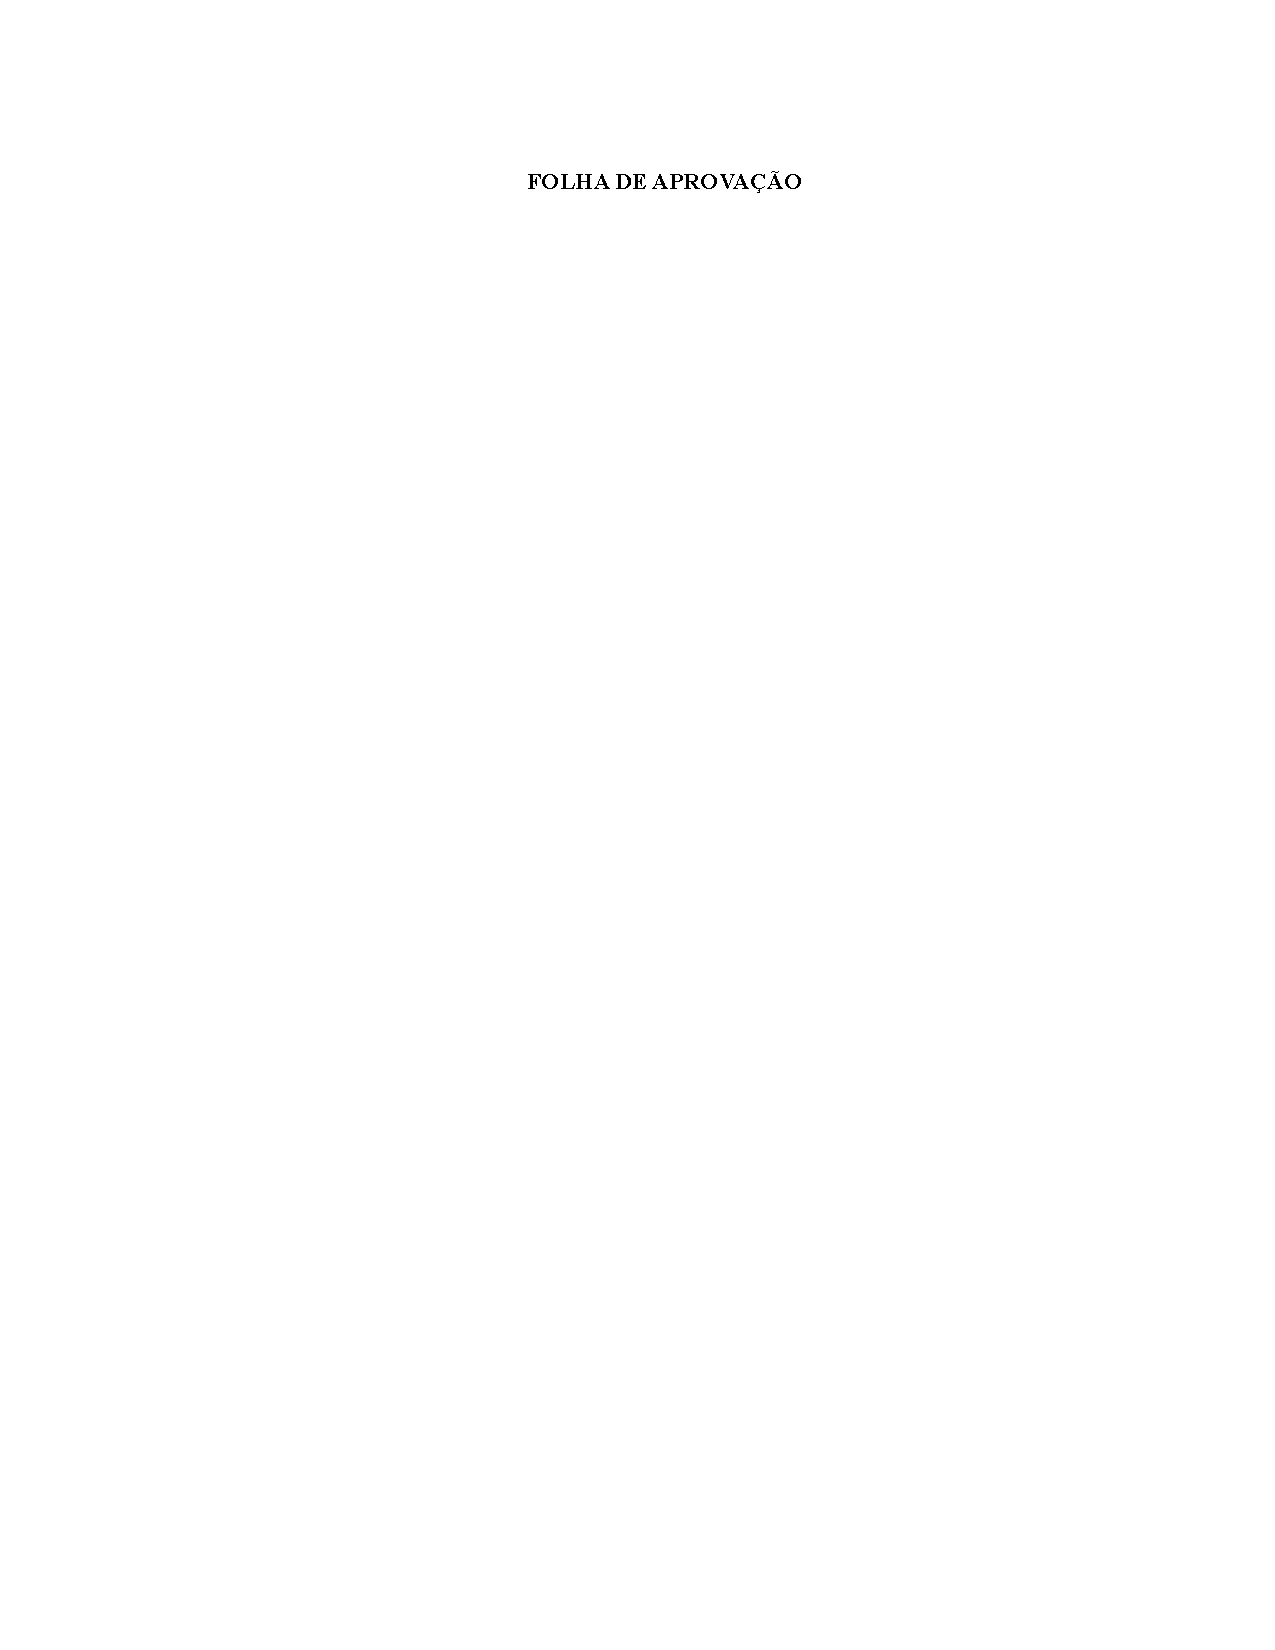
\includepdf[scale=1.0,pages=1]{./PreTexto/folha-aprovacao.pdf} % para adicionar o pdf enviado pelo professor apenas substitua o documento folha-aprovacao.pdf dentro da pasta PreTexto

%% Dedicatória
%% %%%% DEDICATÓRIA
%%
%% Texto em que o autor presta homenagem ou dedica seu trabalho.

\begin{dedicatoria}%% Ambiente dedicatoria

Dedico esta monografia a todas as pessoas que desempenharam papéis essenciais em minha jornada acadêmica e na realização deste trabalho. Em especial, aos meus orientadores, Prof. Dr. Marco Aurélio Graciotto Silva e Prof. Dr. Rodrigo Campiolo, cuja orientação e feedback inestimáveis foram fundamentais para o sucesso deste projeto. Ao meu pai, Manoel Campos, minha maior inspiração na vida, cujo apoio inabalável e palavras de incentivo foram um fator motivador crucial. Às pessoas que, de diversas maneiras, contribuíram para esta pesquisa, o meu profundo agradecimento. Esta monografia é uma homenagem a todos vocês.

\end{dedicatoria}
%% Comente para remover este item

%% Agradecimentos
%%%% AGRADECIMENTOS
%%
%% Texto em que o autor faz agradecimentos dirigidos àqueles que contribuíram de maneira relevante à elaboração do trabalho.

\begin{agradecimentos}%% Ambiente agradecimentos

Certamente não haveria forma diferente de começar os meus agradecimentos sem expressar minha profunda gratidão ao meu orientador, Prof. Dr. Marco Aurélio Graciotto Silva, e ao co-orientador, Prof. Dr. Rodrigo Campiolo, pelas imensuráveis orientações e feedback constante ao longo deste projeto de pesquisa. A dedicação e apoio de ambos foram fundamentais para o sucesso deste trabalho e por estarem presentes em minha trajetória durante a graduação.

Além disso, quero agradecer ao Prof. Dr. Luiz Arthur, que não esteve diretamente envolvido no projeto, mas que desempenhou um papel crucial como professor, mas também como amigo. Sua amizade e apoio constante tornaram minha jornada de aprendizado uma experiência enriquecedora. Suas conversas e mentorias moldaram minha perspectiva e contribuíram extraordinariamente para o meu crescimento como estudante e como pessoa.

Ao Prof. Dr. Igor Wiese, agradeço seu apoio e sua disposição para compartilhar conhecimento e incentivar minha participação em atividades extracurriculares, abrindo portas que foram fundamentais para o meu desenvolvimento como aluno nessa instituição.

Gostaria também de agradecer a minha namorada, Amanda Carvalho, visto que, todos os dias, ela esteve ao meu lado, oferecendo apoio inabalável, especialmente nos momentos em que duvidava das minhas capacidades, deixando-se sempre disponível para dividir as minhas dores e anseios com ela.

Gostaria de expressar minha profunda gratidão à minha mãe, Márcia Farias, pois, mesmo mantendo pouco contato, sempre esteve preocupada em saber se estou bem e feliz. Agradeço por ser uma fonte inesgotável de amor, por sempre me incentivar a alcançar os meus objetivos que, independente do quão grande possam chegar a ser, sempre me apoiou e nunca duvidou de mim.

Gostaria de enviar um abraço especial aos meus amigos incríveis de Portugal, Bernardo Louro, Diogo Lopes e Simão Farias. Mesmo estando a mais de 7 mil km de distância, vocês fizeram parte de cada passo dessa jornada maluca. Vocês são mais do que amigos; são a prova de que as verdadeiras conexões resistem a qualquer distância. Obrigado por serem parte da minha vida de uma maneira tão única e significativa!

Por último, mas definitivamente não menos importante, dedico um agradecimento especial ao meu pai, Manoel Campos, minha maior inspiração de valor incomensurável. Seu apoio constante e palavras de incentivo não apenas foram um fator motivador crucial, mas também por sempre demonstrar orgulho e apontar que estou no caminho certo. Agradeço sinceramente por ter um pai cuja presença é insubstituível, tornando minha jornada ainda mais significativa.

A todos os que, de alguma forma, contribuíram para a realização desta pesquisa, meu sincero agradecimento.

\end{agradecimentos}
%% Comente para remover este item

%% Epígrafe
%% %%%% EPÍGRAFE
%%
%% Texto em que o autor apresenta uma citação, seguida de indicação de autoria, relacionada com a matéria tratada no corpo do
%% trabalho.

\begin{epigrafe}%% Ambiente epigrafe
Primeira Lei: Um robô não pode ferir um ser humano ou, por omissão, permitir que um ser humano sofra algum mal. Segunda Lei: Um robô deve obedecer as ordens que lhe sejam dadas por seres humanos, exceto nos casos em que tais ordens contrariem a Primeira Lei. Terceira Lei: Um robô deve proteger sua própria existência desde que tal proteção não entre em conflito com a Primeira e Segunda Leis (ASIMOV, Isaac, 1950) - observação: A referência deve ser incluída na lista de referências no final do trabalho.

(elemento opcional)
\end{epigrafe}
%% Comente para remover este item

%% Resumo
%%%% RESUMO
%%
%% Apresentação concisa dos pontos relevantes de um texto, fornecendo uma visão rápida e clara do conteúdo e das conclusões do
%% trabalho.

\begin{resumoutfpr}%% Ambiente resumoutfpr

Este trabalho de pesquisa abordou a evolução do código em \gls{sds} por meio da análise de métricas de código, visando criar exemplos trabalhados aplicáveis ao ensino de \gls{es}. A complexidade inerente aos \gls{sds}, cruciais na infraestrutura digital contemporânea, destaca a necessidade de compreender a evolução do código para formar profissionais qualificados. A pesquisa foi conduzida de maneira exploratória, utilizando uma abordagem qualitativa para investigar a relação entre métricas de código e melhorias em \gls{sds}. A heurística desenvolvida para a seleção de códigos representativos mostrou-se fundamental na criação de exemplos trabalhados que ilustram, de forma prática, a dinâmica da evolução do código em \gls{sds}. A escolha criteriosa de ferramentas, como CK, RefactoringMiner e PyDriller, permitiu uma análise abrangente das métricas de código e das mudanças ao longo do tempo em repositórios relevantes, como Apache Kafka e ZooKeeper. A metodologia adotada possibilitou uma compreensão holística da relação entre métricas específicas e melhorias no código, incorporando elementos qualitativos na análise. Os resultados desta pretendem contribuir para a formação de estudantes e profissionais em \gls{es}, preenchendo uma lacuna na literatura sobre a criação de exemplos trabalhados em \gls{sds}. Ao proporcionar uma compreensão mais profunda da evolução do código em \gls{sds} e oferecer exemplos trabalhados pedagogicamente valiosos, espera-se impactar positivamente o ensino e a prática profissional na área.

\end{resumoutfpr}
%% Comente para remover este item

%% Abstract
%%%% ABSTRACT
%%
%% Versão do resumo para idioma de divulgação internacional.

\begin{abstractutfpr}%% Ambiente abstractutfpr

\end{abstractutfpr}
%% Comente para remover este item

%% Lista de algoritmos
%\incluirlistadealgoritmos%% Comente para remover este item

%% Lista de ilustrações
\incluirlistadeilustracoes%% Comente para remover este item

%% Lista de Fotografias
\incluirlistadefotografias %% Comente para remover este item

%% Lista de Gráficos
\incluirlistadegraficos %% Comente para remover este item

%% Lista de tabelas
\incluirlistadetabelas%% Comente para remover este item

%% Lista de quadros
\incluirlistadequadros

%% Listagem de códigos fonte
\incluirlistadecodigosfonte

%% Lista de abreviaturas, siglas e acrônimos
\incluirlistadeacronimos{glossaries}%% Opções: "glossaries" (pacote) ou "file" (arquivo) ou "none" (desabilita)

%% Lista de símbolos
\incluirlistadesimbolos{nomencl}%% Opções: "nomencl" (pacote) ou "file" (arquivo) ou "none" (desabilita)

%% Sumário
\incluirsumario%% Comente para remover este item

%% Formatação de páginas de elementos textuais
\textual%% Não comente esta linha

%%%% CAPÍTULO 1 - INTRODUÇÃO
%%
%% Deve apresentar uma visão global da pesquisa, incluindo: breve histórico, importância e justificativa da escolha do tema,
%% delimitações do assunto, formulação de hipóteses e objetivos da pesquisa e estrutura do trabalho.

%% Título e rótulo de capítulo (rótulos não devem conter caracteres especiais, acentuados ou cedilha)

\chapter{Introdução}\label{cap:introducao}
% Contexto Sistemas Distribuídos.
No cenário atual da computação, os \gls{sds} desempenham um papel fundamental, alimentando a infraestrutura de serviços e aplicações que impulsionam nosso mundo digital. De acordo com \citeonline[p. 968]{TanenbaumDistributedSystemsThirdEdition}, um \gls{sd} é definido como ``Um conjunto de computadores independentes que se apresenta a seus usuários como um sistema único e coerente''. Diante disso, emergem desafios inerentes devido à necessidade de apresentar o sistema ao usuário como uma entidade homogênea, embora, intrinsecamente, o sistema seja constituído por diversas partes heterogêneas. A heterogeneidade abrange diversos aspectos, incluindo variações em termos de rede, hardware, sistemas operacionais, linguagens de programação e implementações realizadas por diferentes desenvolvedores \cite{DistributedSystemsCoulouris}.

% Uso de Sistemas Distribuídos no mundo.
A complexidade inerente aos \gls{sds} os torna um campo desafiador, mas, ao mesmo tempo, altamente relevante na computação moderna. Compreender e lidar com essa heterogeneidade e complexidade é essencial para o desenvolvimento, manutenção e escalabilidade de \gls{sds}. De igual modo, a crescente dependência desses sistemas em nossa sociedade digital torna o estudo de \gls{sds} fundamental para a formação de profissionais capacitados e para o avanço da qualidade do ensino em \gls{es}.

% Preocupações em Sistemas Distribuídos.
Nos \gls{sds}, as preocupações com a segurança dos dados e da comunicação, o desempenho eficiente e a capacidade de manter a operação contínua, mesmo diante de falhas, são instigações extremamente pertinentes. A necessidade de proteger informações sensíveis, garantir tempos de resposta ágeis, garantir que a troca de mensagens seja eficiente e manter a disponibilidade de serviços torna o estudo da evolução do código em \gls{sds} ainda mais vital, uma vez que essas complexidades estão inerentemente ligadas ao código que impulsiona esses sistemas. É nesse contexto que a investigação sobre a evolução do código em \gls{sd} se destaca, proporcionando uma visão valiosa sobre como esses sistemas complexos evoluem para atender às demandas em constante mudança da era digital.

% Educação em Sistemas Distribuídos.
Atualmente, a literatura não oferece estudos suficientes sobre educação em Sistemas Distribuídos. Uma análise do estudo intitulado ``Have We Reached Consensus? An Analysis of Distributed Systems Syllabi'' \cite{HaveWeReachedConsensus} destaca a falta de pesquisas atualizadas nesse campo. Esse estudo identificou que tópicos como Processos e Threads, Replicação, Chamadas de Sistema, Controle de Concorrência, Tolerância a Falhas, Sincronização, Comunicação, entre outros constituem os elementos-chave em cursos de \gls{sds}. No entanto, a carência de pesquisas recentes salienta a importância de investigar a evolução do código em \gls{sds}, especialmente com ênfase na educação, dada a relevância crítica desses sistemas na infraestrutura digital contemporânea.

% Exemplo trabalhado de educação em Sistemas Distribuídos.
O artigo ``Information-Driven Security Analysis Tools and Techniques for the Study and Practice of Security Engineering'' descreve o desenvolvimento contínuo da \textit{SE Workbench}, uma plataforma educacional composta por ferramentas e páginas da web que evoluíram ao longo do tempo. Essas ferramentas, como o \gls{sae}, proporcionam análises de segurança, destacando técnicas e táticas de ataque, auxiliando na documentação de casos anômalos e facilitando a modelagem de ameaças. O \gls{sae}, inserido em um contexto mais amplo de estudo sobre \gls{sds}, oferece uma interface baseada em navegador para analisar, manipular e exportar informações relacionadas à segurança. Esse avanço tecnológico, integrado ao ensino, destaca-se como uma contribuição relevante para abordar preocupações de segurança em \gls{sds}, oferecendo aos estudantes e profissionais recursos educacionais significativos no campo da segurança cibernética.
\cite{SecurityAnalysis:2023}

% Exemplos trabalhados em Ciência da Computação.
A eficácia do ensino em Ciência da Computação, particularmente no contexto de \gls{sds} e \gls{es}, está intrinsecamente ligada ao desenvolvimento e uso de exemplos trabalhados (do inglês, \textit{worked example}). Um exemplo trabalhado é uma ferramenta pedagógica poderosa, definida como um trabalho cognitivo e experimental que oferece uma solução ideal e praticável para um problema específico, permitindo que aprendizes examinem e aprendam com a solução proposta \cite{Robert.Atkinson-etal:2000}. A literatura destaca a importância dos exemplos trabalhados na disseminação de conceitos e padrões, fornecendo uma solução de estado da arte para um tópico específico. A falta de pesquisa dedicada aos exemplos trabalhados nesta área é evidente, e muitos professores enfrentam obstáculos ao incorporar exemplos reais em suas práticas pedagógicas \cite{Simone.Tonhao-etal:2021}.

% Exemplos trabalhados na Engenharia de Software.
No âmbito da \gls{es}, os exemplos trabalhados frequentemente assumem a forma de apresentação passo a passo da execução de códigos específicos. Esses exemplos, quando elaborados com alta qualidade, incorporam elementos essenciais como ``\textit{inter-example feature}'' e ``\textit{intra-example feature}'' \cite{Robert.Atkinson-etal:2000}. No entanto, pesquisas indicam a escassez de estudos específicos sobre exemplos trabalhados na Ciência da Computação, uma vez que tarefas de programação exigem alto teor cognitivo \cite{Skudder-LuxtonReilly:2014}. Além disso, estratégias como ``\textit{Faded Worked Examples}'', que envolvem a apresentação gradual de exemplos resolvidos, têm mostrado impacto significativo na aprendizagem, promovendo a abstração do aluno e desenvolvendo a capacidade de recuperar informações \cite{Skudder-LuxtonReilly:2014}.

\section{Objetivos}\label{sec:objetivos}
\subsection{Objetivo geral}\label{subsec:objetivoGeral}
% Objetivo Geral.
 Neste contexto, o objetivo geral deste projeto de pesquisa é desenvolver uma heurística para identificar exemplos de código-fonte representativos do aprimoramento do \textit{software} de um \gls{sd} por meio da análise de métricas de código usadas na \gls{es}. Essa heurística será projetada para auxiliar na seleção de exemplos trabalhados que demonstrem como o código em \gls{sds} se adaptam e evoluem ao longo do tempo. Em decorrência disso, uma vez conquistada a heurística almejada, objetiva-se criar um exemplo trabalhado, de modo a compreender por que um código específico atende às métricas de código desejadas no âmbito do desenvolvimento de software.

\subsection{Objetivos específicos}\label{subsec:objetivosEspecificos}
% Objetivos Específicos.
\begin{itemize}
    \item Desenvolver uma heurística de seleção que possa analisar as métricas de código
    \item Identificar exemplos de código-fonte que representem eficazmente a evolução em \gls{sds} ao longo do tempo.
    \item Fornecer um exemplo trabalhado para a \gls{es}, identificando em quais aspectos um determinado código evoluiu, reconhecendo padrões, desafios comuns e práticas recomendadas.
\end{itemize}

\section{Justificativa}\label{sec:justificativa}
% Motivo de usar Sistemas Distribuídos como objeto de estudo.
A complexidade e heterogeneidade inerentes aos \gls{sds} estabelecem desafios significativos para o desenvolvimento, manutenção e escalabilidade desses sistemas. Compreender e abordar essas complexidades é crucial, dada a dependência crescente dos \gls{sds} em nossa sociedade digital. A dependência abrange desde redes sociais até sistemas de transporte, saúde e muito mais. Portanto, para conquistar uma boa formação de estudantes e profissionais na área da Computação, faz-se necessário o entendimento de \gls{es} e \gls{sds}, tornando-se uma necessidade iminente para atender à demanda crescente por profissionais qualificados nesse campo. É nesse contexto que a investigação sobre a evolução do código em \gls{sds} assume destaque. O estudo visa proporcionar uma compreensão mais profunda de como o código-fonte em \gls{sds} se adapta ao longo do tempo para atender às demandas da era digital em constante evolução.

% Objetivos do trabalho.
Os objetivos traçados neste trabalho se alinham com a necessidade de abordar essas complexidades. O desenvolvimento de uma heurística para identificar exemplos de código-fonte representativos da evolução em \gls{sds} contribuirá para a formação de estudantes e profissionais em \gls{es}. Esses exemplos servirão como valiosos recursos de ensino e estudo, facilitando a compreensão das complexidades e desafios dos \gls{sds} em um ambiente distribuído e interconectado.

% Justificativa Geral.
Portanto, a justificativa para este estudo se baseia na importância crítica de compreender a evolução do código em \gls{sds}, contribuindo para a formação de profissionais mais capacitados e avançando a qualidade do ensino em \gls{es}. Este estudo procura preencher uma lacuna na literatura sobre a criação de exemplos trabalhados em \gls{sds} para ser objeto de estudo na \gls{es}, fornecendo percepções valiosas para o desenvolvimento e manutenção de \gls{sds} e aprimorando a prática profissional neste campo essencial da computação.

% Lacuna na literatura.
Os estudos existentes, como ``Students' Perception of Example-Based Learning in Software Modeling Education'' \cite{Tiago.Bonetti-etal:2023}, ``Learning from Examples - Instructional Principles from the Worked Examples Research'' \cite{Robert.Atkinson-etal:2000} e ``Using Real Worked Examples to Aid Software Engineering Teaching' \cite{Simone.Tonhao-etal:2021} e ``Uma Plataforma Gamificada de Desafios Baseados Em \textit{Worked Examples} Extraídos de Projetos de Software Livre Para o Ensino de Engenharia de Software'' \cite{Simone.Tonhao-etal:2022} comprovam que o uso de exemplos trabalhados, quando aplicados corretamente, potencializam severamente o engajamento e retenção do conteúdo exposto, porém maioria desses trabalhos são muito focado apenas na \gls{es}. Além disso, o trabalho ``DistFax - A Toolkit for Measuring Interprocess Communications and Quality of Distributed Systems''\cite{DistFax} já tem um cunho de análise de métricas em \gls{sds}, porém não com o intuito de criar um exemplo trabalhado, mas sim de fornecer uma ferramente que ajuda analisar determinados aspectos de \gls{sds}. Dessa forma, até o momento, não foram encontradas pesquisas sobre a utilização da evolução de códigos de Sistemas Distribuídos por meio de métricas estáticas de código para a criação de exemplos trabalhados na disciplina de Engenharia de Software.

% Possíveis ameaças a viabilidade desta pesquisa.
Em projetos de desenvolvimento de software, a qualidade e organização dos dados desempenham um papel crucial na condução de pesquisas significativas. No entanto, um dos fatores que podem inviabilizar a pesquisa seria enfrentar com a presença de dados excessivamente poluídos. Isso pode ocorrer quando os \textit{commits} de código, responsáveis por registrar alterações no software, não são adequadamente divididos e agregam uma quantidade substancial de refatorações em um único \textit{commit}, muitas vezes não diretamente relacionadas à mensagem do mesmo.

\section{Estrutura do trabalho}
\label{sec:estruturaTrabalho}

% Estrutura do trabalho.
A estrutura desta monografia segue uma abordagem organizada, dividida em seções fundamentais para uma compreensão abrangente do trabalho. Inicia-se com a introdução, apresentando o contexto e os objetivos da pesquisa. O referencial teórico abrange a fundamentação teórica essencial e revisão de trabalhos relacionados, proporcionando a base conceitual necessária. A metodologia detalha a abordagem proposta, incluindo questões da pesquisa, ferramentas, métodos e um cronograma claro para orientar a condução da pesquisa. Os resultados esperados antecipam a análise das métricas obtidas dos projetos selecionados. Finalmente, a seção de conclusões oferece uma síntese dos principais resultados, mencionando as limitações do estudo. Essa estrutura visa fornecer uma visão completa e lógica do desenvolvimento e conclusão deste trabalho de pesquisa.

%%%% CAPÍTULO 2 - REVISÃO DA LITERATURA (OU REVISÃO BIBLIOGRÁFICA, ESTADO DA ARTE, ESTADO DO CONHECIMENTO)
%%
%% O autor deve registrar seu conhecimento sobre a literatura básica do assunto, discutindo e comentando a informação já publicada.
%% A revisão deve ser apresentada, preferencialmente, em ordem cronológica e por blocos de assunto, procurando mostrar a evolução do tema.
%% Título e rótulo de capítulo (rótulos não devem conter caracteres especiais, acentuados ou cedilha)
\chapter{Referencial teórico}
\label{cap:referencialTeorico}


\section{Fundamentação teórica}
\label{section:background}
Falar sobre \gls{sds} usando o \cite{DistributedSystemsCoulouris} como base

\subsection{Exemplos trabalhados}

% Definição de exemplo trabalhado
A definição de exemplo trabalhado encontra-se claramente difundida na literatura, passível de ser compreendido como um trabalho cognitivo e experimental com o intuito de fornecer uma solução ideal, todavia próxima ao praticável, para um problema específico, no qual uma pessoa com escasso ou nenhum conhecimento acerca do tema possa examinar e aprender com a solução proposta. Sendo assim, o desenvolvimento e estudo de exemplos trabalhados enriquecem a qualidade do que é lecionado em sala de aula, uma vez que a solução ideal pode representar muito bem o estado da arte para um determinado tópico, visto que dissemina conceitos e padrões do problema apresentado \cite{Robert.Atkinson-etal:2000}.

% Definição de exemplo trabalhado em educação em computação
\cite{Skudder-LuxtonReilly:2014}

% Exemplos trabalhos para engenharia de software
\cite{Simone.Tonhao-etal:2021}
\cite{Simone.Tonhao-etal:2022}
\cite{Tiago.Bonetti-etal:2023}


\subsection{Métricas de software}

A Metrics Suite for Object-Oriented Design.
\cite{MetricsSuite}

\begin{itemize}
    \item \gls{cbo}: Consiste na definição do grau de acoplamento (dependências) que uma determinada classe apresenta. Quanto maior for o valor do \gls{cbo}, maior é o grau de acoplamento da classe, o que indica maior interdependência entre classes. Isso pode tornar o código mais complexo e menos flexível, uma vez que alterações na classe afetaria o comportamento de inúmeras outras classes. Dessa forma, para um determinado código, dada a sua evolução, quando observada uma queda nesse valor, tem-se então um bom indício de melhorias relevantes na qualidade daquele código.
    \item \gls{cbom}: Métrica similar a anterior, todavia considera também a dependência de classes uma referência a um objeto do tipo, ou seja, ao adicionar uma simples chamada de um método da classe, essa métrica é incrementada. Intuitivamente, o \gls{cbom} foi utilizado nos estágios iniciais do estudo foi retirado por poluir os valores, visto que o escopo de refatorações nas métricas foi menos restrito a refatorações da classe ou do método.
    \item \gls{rfc}: Refere-se ao número de invocações únicas de um método de uma determinada classe, isto é, a métrica conta o número de invocações estáticas. 
    OBS: Analisar e explicar o impacto dos valores dessa métrica.
    \item \gls{wmc}: OBS: Analisar e explicar o impacto dos valores dessa métrica de acordo com \cite{MetricsSuite}
\end{itemize}

\subsection{Educação em sistemas distribuídos}


\section{Trabalhos relacionados}
\label{section:related-work}

DistFax: A Toolkit for Measuring Interprocess Communications and Quality of Distributed Systems.
\cite{DistFax}

%%%% CAPÍTULO 3 - Metodologia

\chapter{Metodologia}\label{cap:Metodologia}
Este capítulo delineia os objetivos e a abordagem da pesquisa, apresentando uma visão geral das questões fundamentais apresentadas. Além disso, não só explica as métricas, ferramentas, repositórios utilizados, como também o método e resultados esperados, relacionados com o cronograma definido para a conclusão do projeto de pesquisa.

% Questões da pesquisa.
\section{Questões de pesquisa}
As questões de pesquisa foram formuladas com base nos objetivos geral e específicos desta monografia. Elas direcionarão a investigação sobre a evolução de projetos de \gls{sds} por meio da análise de métricas de código, de modo a criar um exemplo trabalhado para a \gls{es}, como apresentadas abaixo:

% Questões da pesquisa.
\begin{enumerate}
    \item Como identificar métricas de qualidade de código relevantes para a análise da evolução em \gls{sds}?
    
    \item Quais são os padrões e tendências observados que correspondem a uma melhoria clara do código em \gls{sds}?
    
    \item Como as melhorias de código se refletem nas métricas selecionadas e qual é a relação delas com características não funcionais como acoplamento, coesão, reusabilidade e manutenibilidade?
    
    \item Quais são as métricas e características mais relevantes para a seleção de exemplos de código apropriados para a criação de exemplos trabalhados na \gls{es}?
\end{enumerate}

% Abordagem Proposta.
\section{Abordagem proposta}

O presente trabalho propõe o desenvolvimento de uma heurística para identificar exemplos de código-fonte representativos da melhoria da qualidade de software em \gls{sds}, por meio da análise de métricas de código utilizadas na \gls{es}. A heurística visa auxiliar na seleção de trechos de código que permitam a criação de exemplos trabalhados que demonstrem como o código em \gls{sds} se adapta e evolui ao longo do tempo.

A heurística a ser desenvolvida nesta pesquisa baseia-se nas melhorias que podem ser identificadas através das métricas selecionadas. As métricas devem ser capazes de capturar informações valiosas relacionadas à evolução do código em \gls{sds}. Logo, são empregadas ferramentas específicas em repositórios de código aberto cuidadosamente selecionados. 

% Métricas CK.
\subsection{Métricas de software} \label{sec:metricasDeSoftware}
O artigo ``\textit{A Metrics Suite for Object Oriented Design}''\cite{MetricsSuite} apresenta um conjunto de métricas para avaliação do design de código orientado a objetos, introduzindo métricas que permitem compreender a complexidade e qualidade do código-fonte. As principais métricas apresentadas no artigo são listadas a seguir.

% Explicação das Métricas CK.
\begin{itemize}
    \item \textbf{\gls{cbo}}: Reflete o grau de acoplamento, ou seja, as dependências que uma classe específica possui, indicando a quantidade de classes diretamente associadas a ela, já que utiliza métodos dessas classes. Um valor elevado sugere maior complexidade e menor flexibilidade, pois mudanças na classe podem impactar várias outras. Não suficiente, demasiado acoplamento diminui o grau de modularidade de uma classe. Observar uma redução no \gls{cbo} ao longo da evolução do código é um indicativo positivo de melhorias na qualidade do código. Um esforço para reduzir o \gls{cbo} pode levar a um \textit{design} de \textit{software} mais modular, onde as mudanças em uma parte do sistema têm menos probabilidade de exigir mudanças em outra.
    
%    Uma variação da implementação do \gls{cbo}, também denominada \gls{cbom} considera a dependência de classes como uma referência a um objeto do mesmo tipo. Isso significa que, ao adicionar uma simples chamada de método da classe, a métrica é incrementada. 

    \item \textbf{\gls{dit}}: Reflete a profundidade da árvore de herança à qual uma classe depende, indicando a quantidade de ancestrais que uma classe tem. Um valor elevado de \gls{dit} pode indicar uma maior complexidade e potencial para efeitos colaterais ao realizar alterações em alguma das superclasses.
    
    \item \textbf{\gls{lcom}}: Representa o coeficiente de falta de coesão em métodos, mensurando a coesão em uma classe. O valor varia de 0 a 1, onde 0 indica alta coesão e 1 indica falta de coesão. Baixos valores são desejados, indicando que os métodos estão fortemente inter-relacionados, contribuindo para uma classe mais coesa.

    \item \textbf{\gls{noc}}: Indica o número de filhas diretas de uma classe. Um valor alto pode indicar maior reusabilidade. Isso implica que a referida classe desempenha uma função importante, dada a dependência de outras classes sobre ela.

    \item \textbf{\gls{rfc}}: Refere-se ao tamanho do conjunto de respostas de uma classe, ou seja, o número de métodos que podem ser potencialmente executados em resposta a uma mensagem recebida por um objeto dessa classe. Um valor menor de \gls{rfc} indica que uma classe tem menos comportamentos e, potencialmente, um menor grau de complexidade. Classes com \gls{rfc} baixo tendem a ser mais coesas e menos acopladas, pois interagem com menos outras classes e componentes, facilitando assim a manutenção e a testabilidade.

    \item \textbf{\gls{wmc}}: Simboliza a soma dos valores de complexidade dos métodos de uma classe específica. Um valor elevado indica que a classe pode ser complexa, com múltiplos métodos, implicando em um custo significativo para o desenvolvimento e manutenção. Além disso, a existência de vários métodos associados a uma classe sugere que ela pode ser menos genérica, sem mencionar o possível impacto nos filhos dessa classe. Classes com \gls{wmc} baixo tendem a ser mais coesas, o que significa que elas têm um propósito bem definido e limitado. A redução do \gls{wmc} pode ser um sinal de que a classe está se tornando mais focada em suas responsabilidades, o que facilita o entendimento, a manutenção e a extensão do código.
\end{itemize}

% Ferramentas Utilizadas e o motivo.
\subsection{Ferramentas}\label{sec:ferramentas}
% Ferramenta CK.
O \gls{ck}\footnote{https://github.com/mauricioaniche/ck}\cite{aniche-ck} é a ferramenta utilizada nesta pesquisa para analisar a qualidade do código-fonte em projetos Java\cite{JavaProgrammingLanguage} por meio de métricas estáticas. Essas métricas fornecem informações valiosas sobre características como complexidade, acoplamento e coesão de classes. A ferramenta em questão apresenta mais de 35 métricas.

% Ferramenta RefactoringMiner.
O \textit{RefactoringMiner}\footnote{https://github.com/tsantalis/RefactoringMiner}\cite{Tsantalis:ICSE:2018:RefactoringMiner} é uma ferramenta no contexto da \gls{es}, especializada em identificar e analisar refatorações de código-fonte. Essa ferramenta fornece uma compreensão aprofundada das mudanças realizadas em um código ao longo do tempo. Com a sua capacidade de reconhecer padrões de refatoração, o \textit{RefactoringMiner} permite que os desenvolvedores analisem como o código foi modificado, de modo a melhorar a qualidade, manutenibilidade e eficiência do software.

% Ferramenta PyDriller.
A biblioteca \textit{PyDriller}\footnote{https://github.com/ishepard/pydriller}\cite{PyDrillerSpadini2018}, disponível para a linguagem de programação Python, é um recurso para análise de repositórios. Sua funcionalidade possibilita aos pesquisadores e desenvolvedores explorar e compreender a evolução do código em projetos Python de uma maneira eficiente. O \textit{PyDriller} oferece recursos para extrair informações, como histórico, autoria e mensagens de \textit{commits}, além de detalhes específicos do estado do código em um determinado momento, contribuindo assim para a pesquisa e prática em \gls{es} no contexto de sistemas complexos e interconectados.

% Repositórios.
\subsection{Repositórios}\label{sec:repositorios}
A seguir são apresentados os projetos de código aberto disponíveis no https://github.com, que serão analisados neste trabalho de pesquisa.

% Conceito do Apache Kafka.
O \textit{Apache Kafka}\cite{KafkaGitHub} é um sistema de mensagens distribuídas, baseado no modelo \textit{publish-subscribe}, amplamente utilizado em infraestruturas de processamento de eventos em tempo real. Conforme o artigo ``\textit{Apache Kafka: Next Generation Distributed Messaging System}''\cite{ApacheKafkaNextGenerationDistributedMessagingSystem:2010}, o Kafka é projetado para lidar com fluxos de dados em grande escala, permitindo que organizações processem, armazenem e transmitam dados de maneira eficiente, operando em um modelo de log distribuído, no qual as mensagens são registradas em logs (ou tópicos) que podem ser divididos em partições. 
A estrutura do Apache Kafka é composta por vários componentes, incluindo:

% Elementos estruturais do Apache Kafka.
\begin{itemize}
  \item \textbf{Tópicos}: São canais de mensagens nos quais os dados são publicados e armazenados.
  \item \textbf{Produtores}: São responsáveis por publicar mensagens em tópicos do Kafka.
  \item \textbf{Partições}: Os tópicos podem ser divididos em partições para permitir a distribuição e o processamento paralelo de mensagens.
  \item \textbf{Corretores (Brokers)}: São servidores que armazenam e distribuem as mensagens. Eles desempenham um papel central na arquitetura do Kafka.
  \item \textbf{Consumidores}: São aplicativos que se inscrevem nos tópicos para receber mensagens e processá-las.
  \item \textbf{\gls{zk} (KRaft em 2023)}: No passado, o Kafka dependia do Apache \gls{zk} para gerenciamento de metadados e coordenação. No entanto, em 2023, o Kafka adotou o \textit{KRaft} como substituto, eliminando a dependência do \gls{zk}, com o intuito de deixá-lo mais simples e robusto.
\end{itemize}

% Implicações da estrutura do Kafka.
Essa arquitetura permite a escalabilidade, tolerância a falhas e a distribuição das mensagens em várias máquinas e servidores, tornando-o uma escolha popular em empresas como LinkedIn, X (Twitter), Uber, Foursquare, entre outros para a construção de pipelines de dados em tempo real e sistemas de processamento de eventos\cite{KafkaPoweredBy}. Dessa forma, dada a sua arquitetura, uso no mundo real, além da capacidade do \textit{``Apache Kafka''} lidar com volumes massivos de dados em tempo real, ele torna-se um ótimo candidato a ser estudado.

% Conceito do ZooKeeper.
O \gls{zk}\cite{ZookeeperGitHub} é um serviço de coordenação distribuída amplamente utilizado para sistemas de grande escala na internet. Ele fornece um ambiente confiável e altamente disponível para a coordenação de tarefas entre diversos nós em um cluster distribuído. Na ótica do artigo ``\textit{ZooKeeper: Wait-free coordination for Internet-scale systems}''\cite{ZooKeeperWaitFree:2010}, o \gls{zk} é baseado em um conjunto de servidores distribuídos que formam o chamado ``\textit{ensemble}''. Cada servidor nesse conjunto mantém uma cópia completa dos dados de configuração e estado do sistema. Os clientes se conectam a qualquer servidor do conjunto e podem ler ou gravar informações. Quando os clientes gravam informações, elas são replicadas para a maioria dos servidores no conjunto antes de serem confirmadas, garantindo assim a consistência dos dados. 

% Conceito do ZooKeeper - Continuação.
O \gls{zk} fornece um sistema de coordenação sem espera (do inglês, ``\textit{wait-free}''), por meio de um mecanismo de observação para permitir que os clientes armazenem dados em \textit{cache} sem ter que gerenciar o \textit{cache} do cliente diretamente. Além disso, a implementação do algoritmo denominado \gls{zab} é responsável por garantir a consistência de dados distribuídos no \gls{zk} por meio do uso do \textit{Two-Phase Commit Protocol} para replicar todas as transações para todos os nós do cluster do \gls{zk}\cite{CloudKarafkaZAB}. O \textit{Two-Phase Commit Protocol} consiste em duas fases. Na primeira fase, um coordenador propõe a execução de uma transação aos participantes, que respondem indicando se estão prontos para realizar a transação. Na segunda fase, se todos concordarem, o coordenador emite o comando de \textit{commit} para que os participantes realizem efetivamente a transação; caso contrário, emite o comando de \textit{rollback}, revertendo as alterações. 

O \textit{``ZooKeeper''} é utilizado para coordenação e gerenciamento de serviços distribuídos. Ele oferece um serviço de consenso altamente confiável para \gls{sds}, garantindo a consistência e a sincronização entre os nós. Essa funcionalidade permite a implementação de serviços distribuídos confiáveis e escaláveis, tornando o \textit{``ZooKeeper''} uma escolha valiosa para este estudo.

% Métodos.
\section{Métodos}\label{sec:metodo}
Este trabalho de pesquisa adota uma abordagem exploratória com o propósito de desenvolver uma heurística que possibilite a seleção criteriosa de códigos representativos de melhorias de software, de acordo com métricas específicas de \textit{código} em projetos de \gls{sds}. O objetivo principal é aprofundar a compreensão desses casos, proporcionando uma análise detalhada da evolução do código em resposta a mudanças nas métricas escolhidas. Esse estudo visa contribuir diretamente para a construção de exemplos trabalhados aplicáveis ao contexto da \gls{es}.

A natureza exploratória da pesquisa pretende proporcionar uma visão mais ampla sobre como as métricas de código em projetos de \gls{sds} refletem melhorias significativas. A heurística em desenvolvimento visa identificar casos exemplares de evolução de código, considerando métricas específicas, selecionadas com base nas melhores práticas e no entendimento profundo das características inerentes aos \gls{sds}.

Para alcançar esses objetivos, serão realizadas análises minuciosas de repositórios de código aberto relevantes na área de \gls{sds}, considerando não apenas a evolução do código-fonte, mas também as mudanças nas métricas escolhidas ao longo do tempo. Na esfera da segurança, será explorada a possibilidade de correlacionar informações com alterações específicas no código, proporcionando uma análise abrangente e multifacetada. Não suficiente, questões como IPC, disponibilidade, transparência e heterogeneidade também serão estudadas. A metodologia adotada permite, assim, uma compreensão holística da relação entre a qualidade do código e as métricas específicas selecionadas.

Além disso, a pesquisa visa ir além da mera análise quantitativa, incorporando uma abordagem qualitativa ao desenvolver exemplos trabalhados que demonstrem, de forma clara e pedagogicamente eficaz, como a evolução do código em \gls{sds} pode ser interpretada e compreendida no âmbito da \gls{es}. Essa abordagem qualitativa permite a construção de um conhecimento prático e aplicável que possa enriquecer o ensino e a prática profissional na área.

\section{Resultados esperados e cronograma}

% Passo a passo e resultados esperados.
\begin{enumerate}
    \item Realizar uma revisão da literatura, explorando estudos sobre métricas de código em \gls{es} e \gls{sds}.
    \\\textbf{Resultado esperado:} Lista de estudos sobre exemplos trabalhados e as respectivas contribuições.

    \item Selecionar um ou mais repositórios \textit{open-source} pertinentes à área de \gls{sds} que servirão como fonte de exemplos de código para análise.
    \\\textbf{Resultado esperado:} Lista de repositórios \textit{open-source} ativamente mantidos e utilizados em aplicações reais selecionados para análise.

    \item Selecionar métricas de código específicas e relevantes apropriadas para avaliar a evolução de código em \gls{sds}, considerando as melhores práticas da área.
    \\\textbf{Resultado esperado:} Lista de métricas de código selecionadas, capazes de refletir melhorias, por exemplo, com relações ao acoplamento e coesão de cada classe.

    \item Escrita e publicação de um artigo resumido no evento EduComp2024 sobre o projeto e as metodologias utilizadas até o momento.
    \\\textbf{Resultado esperado:} Resumo publicado apresentando o projeto, metodologias e atividades desenvolvidas de fevereiro até abril no EduComp2024.

    \item Selecionar exemplos específicos de código trabalhados nos repositórios escolhidos, aplicando a heurística desenvolvida e justificando a seleção com base em métricas de código.
    \\\textbf{Resultado esperado:} Lista de candidatos potenciais com refatorações significativas, com relação à evolução da qualidade do código.

    \item Avaliar a utilidade educacional dos exemplos de código selecionados, usando-os em um contexto de ensino.
    \\\textbf{Resultado esperado:} Contribuir para o estudo do código de um \gls{sd} no âmbito da \gls{es}.

    \item Escrita e publicação de um artigo no \textit{SBES-Education} sobre os resultados obtidos até o momento, destacando descobertas e contribuições.
    \\\textbf{Resultado esperado:} Artigo publicado apresentando os resultados e contribuições entre abril e junho no \textit{SBES-Education}.
\end{enumerate}

Dessa forma, a Tabela~\ref{table:schedule} apresenta um cronograma de atividades.

\begin{table}[h]
\centering
\caption{Cronograma de atividades}
\label{table:schedule}
\begin{tabular}{lcccccc}
Atividade/Mês & Jan & Fev & Mar & Abr & Mai & Jun  \\
\hline
1 - Revisão da literatura & x & x & x & x & & \\
2 - Seleção de repositórios & x & x & & & & \\
3 - Seleção de métricas & x & x & x & & & \\
4 - Submissão de um resumo no EduComp2024 & & x & x & x & & \\
5 - Seleção de exemplos & & & & x & x & x \\
6 - Avaliação da utilidade educacional & & & & x & x & x \\
7 - Submissão de um artigo no \textit{SBES-Education} & & & & & x & x
\end{tabular}
\end{table}

\chapter{Resultados Prévios}
\label{cap:resultados}

% Seleção de Projetos.
\section{Seleção de projetos}

% Critérios de seleção de repositórios.
Os critérios para a seleção de repositórios foram determinados pelos seguintes fatores:

\begin{itemize}
    \item \textbf{Ser um repositório Java:} Essencial para viabilizar a aplicação das métricas \gls{ck}.
    \item \textbf{Ser de código aberto (\textit{open-source}):} A escolha por repositórios abertos, hospedados em plataformas como o \textit{Github}, visa garantir a transparência e acessibilidade do código-fonte.
    \item \textbf{Ser ativamente mantido e atualizado:} A ativa manutenção é crucial para garantir que os repositórios estejam alinhados com as práticas e avanços mais recentes.
    \item \textbf{Ser utilizado em aplicações do mundo real:} A seleção de repositórios empregados em contextos práticos proporciona uma análise mais relevante e aplicável às situações reais.
\end{itemize}

Os projetos escolhidos foram o \textit{``Apache Kafka''} \cite{KafkaGitHub} e o \textit{``ZooKeeper''} \cite{ZookeeperGitHub}. Essa escolha baseou-se no fato de os repositórios serem projetos \textit{open-source} disponíveis na plataforma GitHub, onde ambos são mantidos e atualizados de forma ativa para serem utilizados em ambientes do mundo real. Além disso, esses projetos lidam com questões altamente relevantes em \gls{sds}.

Logo, ambos os repositórios têm muito a agregar em termos de implementação e evolução, tanto para a área de \gls{sds} quanto para a \gls{es}. Assim, a escolha desses repositórios permite a análise da evolução do código em contextos práticos e desafiadores, contribuindo para uma compreensão mais abrangente das práticas de desenvolvimento em \gls{sds}.

% Métricas selecionadas inicialmente.
\section{Métricas Preliminarmente Selecionadas}

No estágio inicial desta pesquisa, optou-se por selecionar um conjunto específico de métricas, incluindo \gls{cbo}, \gls{cbom}, \gls{rfc} e \gls{wmc}. Essa escolha foi motivada pela intenção de obter uma combinação abrangente que abordasse diferentes aspectos da qualidade do código. As métricas \gls{cbo} e \gls{cbom} foram escolhidas para fornecer \textit{insights} sobre o nível de acoplamento em classes ou métodos, enquanto \gls{rfc} foi selecionada para medir o grau de comunicação entre os elementos do código. Por fim, a métrica \gls{wmc} foi incluída para avaliar a complexidade dos métodos em uma classe.

Contudo, durante o desenvolvimento do estudo, decidiu-se remover a métrica \gls{cbom} da análise. Essa decisão foi tomada devido à percepção de que a inclusão de \gls{cbom} poderia introduzir poluição nos dados, aumentando a complexidade artificialmente. Isso ocorre, por exemplo, quando a adição de uma chamada a um método da própria classe afeta negativamente a métrica. Dessa forma, a exclusão de \gls{cbom} visou manter a integridade e a precisão das métricas escolhidas, proporcionando uma análise mais clara e objetiva da evolução do código.

% Desenvolvimento das ferramentas disponíveis no GitHub feitas em Python.
\section{Desenvolvimento da ferramenta}

As ferramentas desenvolvidas podem ser encontradas no Github \footnote{https://github.com/BrenoFariasdaSilva/Scientific-Research}, estando as três primeiras no diretório ``\textit{PyDriller}'' e as duas últimas no diretório ``\textit{RefactoringMiner}'', sendo que todas foram feitas usando a linguagem de programação Python \cite{PythonProgrammingLanguage}.

A primeira ferramenta desenvolvida, denominada \textit{code\_metrics.py} \cite{PyDriller:CodeMetrics:2023}, está integrada ao \textit{PyDriller} e ao \gls{ck}. Durante esse processo, a ferramenta percorre toda a árvore de \textit{commits} de um repositório específico. Para cada \textit{commit}, o \gls{ck} é executado, resultando na geração das métricas \gls{ck} para cada estado do repositório ao final da execução. Adicionalmente, a ferramenta produz um \textit{diff} para cada refatoração realizada no repositório, possibilitando a investigação das refatorações realizadas no código em caso de identificação de uma tendência de melhoria das métricas.

A segunda ferramenta desenvolvida, denominada \textit{metrics\_changes.py} \cite{PyDriller:MetricsChanges:2023},  depende da execução da primeira para operar. Essencialmente, esta ferramenta percorre as métricas de todos os estados do repositório processado, produzindo os seguintes resultados:

\begin{itemize}
    \item \textbf{Evolução das métricas}: Geração de arquivos divididos por classe e métodos, contendo o histórico completo de alterações em cada classe ou método, incluindo suas métricas correspondentes.
    \item \textbf{Predição das métricas}: Criação de arquivos segmentados por classe e métodos, apresentando uma predição baseada na regressão linear aplicada às métricas analisadas, utilizando o histórico gerado anteriormente.
    \item \textbf{Estatísticas das métricas}: Produção de um arquivo para classes e outro para métodos, ordenados pelo número de alterações efetuadas em cada classe ou método.
    \item \textbf{Alterações substanciais nas métricas}: Identificação de padrões de decréscimo do \gls{cbo}, oferecendo uma análise detalhada das classes ou métodos que apresentam tendências de melhoria ao longo do tempo.
\end{itemize}

Assim, resumidamente, as ferramentas \textit{code\_metrics.py} e \textit{metrics\_changes.py} geram metadados que facilitam a análise dos códigos, reduzindo o escopo de busca por refatorações que, à luz das métricas, são consideradas relevantes para nosso estudo. Vale ressaltar que, enquanto o estudo que desenvolve o \textit{DistFax} \cite{DistFax} utiliza métricas \gls{ipc} dinâmicas (geradas em tempo de execução), o presente estudo emprega métricas de código estáticas (geradas apenas pela análise do código-fonte). Isso se deve à inadequação das métricas tradicionais para medir a qualidade das trocas de mensagens em \gls{sds}, pois eles não se baseiam em relações explícitas, analisam apenas um computador e não consideram o sistema em sua totalidade. Embora o uso dessas métricas pudesse ser benéfico, o custo computacional pode ser bastante significativo para calcular todas elas.

As figuras a seguir apresentam exemplos das saídas geradas pelo algoritmo \textit{metrics\_changes.py} para a classe \textit{org.apache.zookeeper.server.quorum.Follower}. A seleção dessa classe deve-se ao fato de que, pelo nome, é possível compreender que é uma classe que trata da parte do consenso do protocolo, ou seja, dos participantes (\textit{followers}) entrarem em consenso em uma votação. Dado essa premissa, analisou-se essa classe e percebeu-se uma tendência de queda nas métricas \gls{cbo}, \gls{rfc} e \gls{wmc}.

\begin{figure}[h]
    \centering
    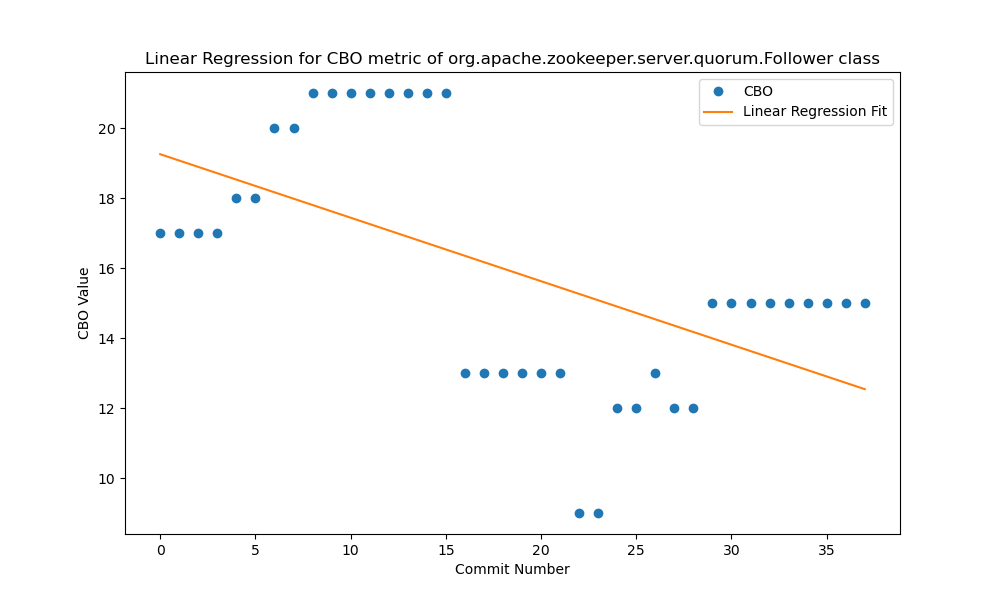
\includegraphics[width=0.8\linewidth]{figuras/Output/Metrics_Predictions/CBO.png}
    \caption{Regressão linear da métrica \gls{cbo} da classe org.apache.zookeeper.server.quorum.Follower}
    \label{fig:RlCBO}
\end{figure}

\begin{figure}[h]
    \centering
    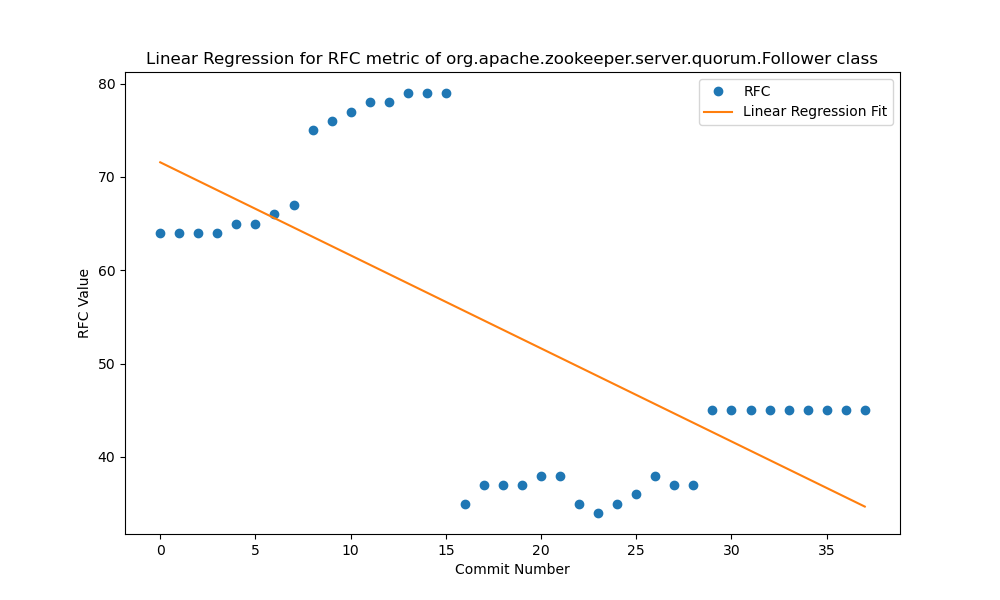
\includegraphics[width=0.8\linewidth]{figuras/Output/Metrics_Predictions/RFC.png}
    \caption{Regressão linear da métrica \gls{rfc} da classe org.apache.zookeeper.server.quorum.Follower}
    \label{fig:RlRFC}
\end{figure}

\begin{figure}[h]
    \centering
    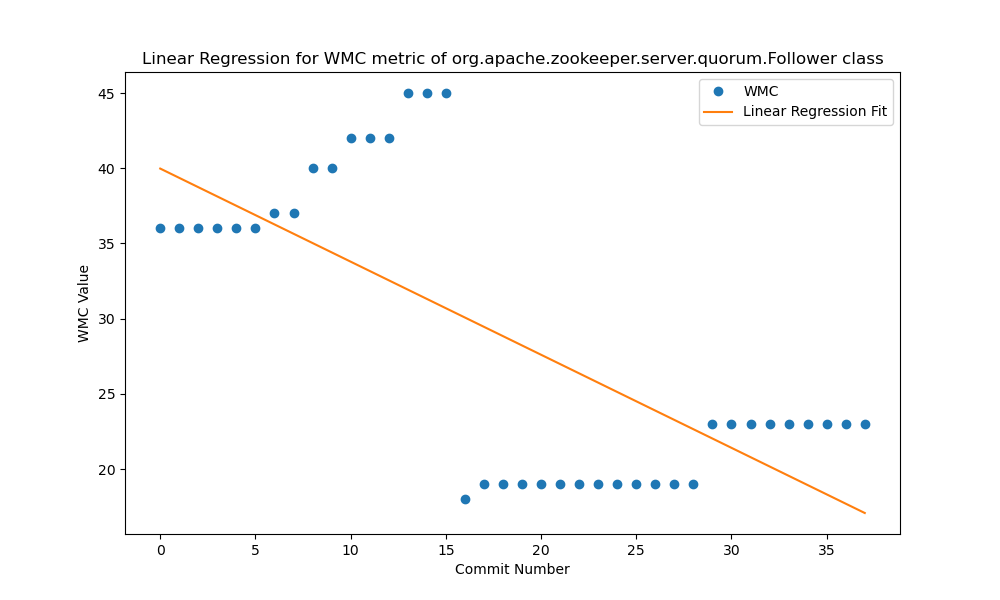
\includegraphics[width=0.8\linewidth]{figuras/Output/Metrics_Predictions/WMC.png}
    \caption{Regressão linear da métrica \gls{wmc} da classe org.apache.zookeeper.server.quorum.Follower}
    \label{fig:RlWMC}
\end{figure}

\begin{figure}[h]
    \centering
    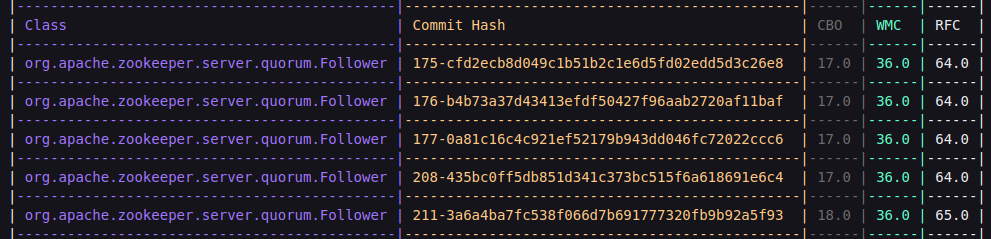
\includegraphics[width=0.8\linewidth]{figuras/Output/Metrics_Evolution/Metrics_Evolution.png}
    \caption{Evolução das métricas da classe org.apache.zookeeper.server.quorum.Follower}
    \label{fig:EvolutionFollowerClass}
\end{figure}

\begin{figure}[h]
    \centering
    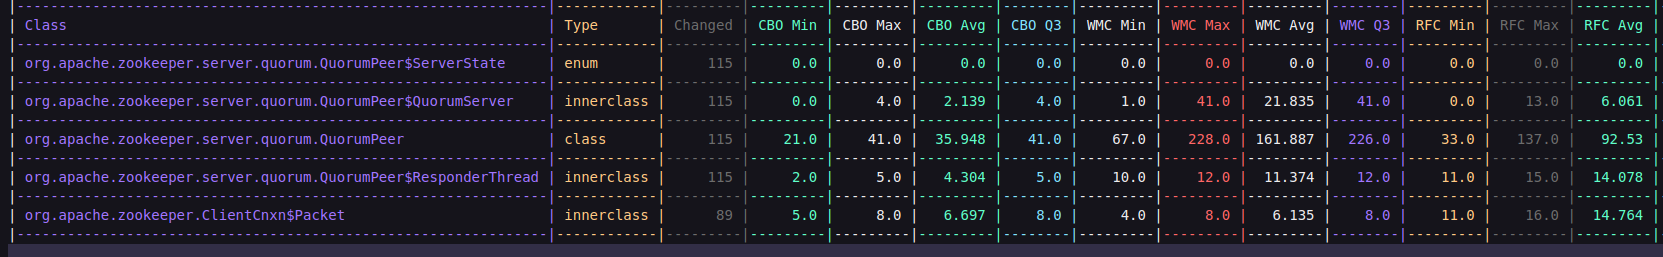
\includegraphics[width=0.8\linewidth]{figuras/Output/Metrics_Statistics/Metrics_Statistics.png}
    \caption{Estatísticas das métricas do ZooKeeper}
    \label{fig:StatisticsFollowerClass}
\end{figure}

As Figuras \ref{fig:RlCBO}, \ref{fig:RlRFC} e \ref{fig:RlWMC} proporcionam uma perspectiva visual das tendências nas métricas \gls{cbo}, \gls{rfc} e \gls{wmc} específicas da classe \textit{org.apache.zookeeper.server.quorum.Follower}. Enquanto isso, as figuras \ref{fig:EvolutionFollowerClass} e \ref{fig:StatisticsFollowerClass} apresentam um vislumbre das cinco primeiras linhas dos \textit{CSVs} gerados, delineando a evolução das métricas de tal classe e as estatísticas gerais das classes no contexto do \textit{ZooKeeper}. As primeiras três imagens oferecem uma compreensão aprofundada do comportamento evolutivo dessa classe específica, enquanto a última concentra-se nas classes mais frequentemente modificadas, destacando sua propensão a refatorações significativas ou sua relevância fundamental dentro do ecossistema do \textit{ZooKeeper}.

A terceira ferramenta desenvolvida, denominada de \textit{track\_files.py} \cite{PyDriller:TrackFiles:2023}, mais uma vez, depende da execução da primeira para funcionar. Em suma, esta ferramenta busca por arquivos específicos nos \textit{diffs} dos repositórios. Neste estudo, ela foi utilizada para localizar arquivos de comentários sobre as refatorações realizadas em um \textit{commit}, como o arquivo ``CHANGES.txt'', uma vez que o espaço da mensagem do \textit{commit} pode oferecer uma visão limitada das refatorações efetuadas.

As ferramentas desenvolvidas, nomeadas \textit{metrics\_evolution\_refactors.py} \cite{RefactoringMiner:RepositoryRefactors:2023} (quarta ferramenta) e \textit{repository\_refactors.py} \cite{RefactoringMiner:MetricsEvolution:2023} (quinta ferramenta),  são substancialmente similares, distinguindo-se apenas no escopo de aplicação, onde a quarta  incide sobre a totalidade do repositório, enquanto a quinta é específica para classes ou métodos dentro do repositório. Ambas as ferramentas compartilham um funcionamento comum, fazendo uso da ferramenta \textit{RefactoringMiner} \cite{Tsantalis:ICSE:2018:RefactoringMiner}.

A utilização das ferramentas associadas ao \textit{RefactoringMiner} é feita por meio da extração do histórico de \textit{commits}, permitindo a análise dos \textit{diffs}, identificando padrões de refatorações. O \textit{RefactoringMiner} possui um banco de dados de refatorações previamente detectadas, permitindo uma análise eficiente das mudanças no código-fonte. A ferramenta gera uma saída estruturada que lista as refatorações identificadas, indicando quais arquivos e linhas de código foram afetados em cada \textit{commit}.

Essa saída estruturada proporciona uma base sólida para análises mais aprofundadas, permitindo uma compreensão detalhada das refatorações realizadas ao longo do tempo. A capacidade de distinguir entre o repositório inteiro (quarta ferramenta) e componentes específicos, como classes ou métodos (quinta ferramenta), amplia a flexibilidade dessas ferramentas, adaptando-as às necessidades específicas de investigação e análise de refatorações em projetos de software.

A saída dos algoritmos que utilizam o \textit{RefactoringMiner} consiste em um objeto \textit{JSON}, semelhante à Figura \ref{fig:RefactoringMinerOutput}, que permite a análise das refatorações por tipo. Destaca-se que, a partir do \textit{JSON} geral, é possível aplicar filtros para armazenar apenas refatorações dos tipos desejados. Essa abordagem proporciona uma visão detalhada e personalizável das transformações efetuadas no código-fonte.

\begin{figure}[h]
    \centering
    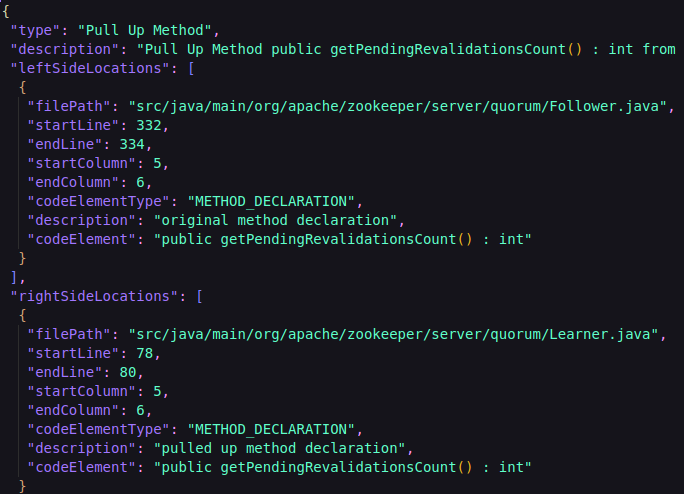
\includegraphics[width=0.8\linewidth]{figuras/Output/RefactoringMiner/org.apache.zookeeper.server.quorum.Learner.png}
    \caption{Refatorações da classe org.apache.zookeeper.server.quorum.Learner}
    \label{fig:RefactoringMinerOutput}
\end{figure}

% Análise das métricas dos projetos selecionados.
\section{Análise das métricas dos projetos selecionados}
Apesar da intenção inicial de analisar dois repositórios, o \textit{``Apache Kafka''} e o \textit{``ZooKeeper''}, até o momento, concentramos nossos esforços exclusivamente no exame do repositório do \textit{``ZooKeeper''}. Esta escolha se fundamenta no tamanho inferior deste repositório em comparação com o \textit{``Apache Kafka''}, permitindo uma análise mais focalizada e a possibilidade de apresentar resultados preliminares neste trabalho. A decisão foi motivada por considerações de limitação de tempo, pois a análise detalhada de um único repositório já representa um desafio significativo, demandando uma abordagem minuciosa para compreender a evolução do código-fonte e as refatorações realizadas.  Neste trabalho, serão mencionados alguns casos analisados que aparentavam ser promissores, no entanto, mostraram algumas dificuldades a mais que iremos lidar nos estágios seguintes deste projeto de pesquisa.

A análise atual revela a presença de vários \textit{commits} no histórico do repositório do \textit{``ZooKeeper''}, e notou-se uma tendência decrescente no valor de métricas, como o \gls{cbo}. No entanto, é crucial observar que apenas uma parcela restrita desses \textit{commits} inclui mensagens associadas a melhorias de desempenho, segurança, substituição de algoritmos ou melhorias de modo geral. 

Lamentavelmente, até o momento, apenas um \textit{commit} apresentou uma correlação direta entre as vulnerabilidades identificadas no banco de dados do \textit{``CVE-Details''} e os \textit{commits} no repositório do \textit{ZooKeeper}. O único caso encontrado foi para o \textit{commit} 9213f7353b1e6ce4d0fdbc1dca963ace1fd32cec, o qual relaciona-se a vulnerabilidade CVE-2021-21295. Entretando, por mais que o \textit{commit} resolva um problema de vulnerabilidade, constatamos que esta refatoração específica consiste apenas na atualização da versão da biblioteca \textit{Netty} no arquivo pom.xml do Java, o qual prove uma estrutura cliente-servidor de E/S não bloqueante, logo ela não se mostra uma boa candidata para correlacionar métricas de código com a segurança, pois se trata de uma ação direta para resolver uma vulnerabilidade conhecida.

A análise do \textit{commit} 83cf0a93c37759334fab885c2010fa0b7d953f52 foi aprofundada, cuja mensagem é ``\textit{ZOOKEEPER-308. Improve the atomic broadcast performance in 3x}''. Apesar da indicação inicial de um ganho de desempenho em 3 vezes, uma investigação mais detalhada revelou que a alteração se limitava à substituição da classe \textit{FileOutputStream''} por \textit{BufferedOutputStream''}. Embora essa mudança resulte em melhoria de desempenho, não constitui uma refatoração significativa, pois o \textit{commit} altera 19 arquivos, sendo relevante apenas o arquivo ``\textit{FileTxnLog.java}'', que consiste na troca das classes mencionadas. Os outros arquivos alterados abordam refatorações relacionadas à validação de objetos nulos antes de operações, mas estão fora do escopo da mensagem do \textit{commit}. Apesar disso, a melhoria de desempenho é reconhecida como válida, embora sua magnitude não possa ser verificada.

Embora a mudança promova efetivamente uma melhoria de desempenho, as métricas tradicionais de código, como \gls{cbo}, \gls{rfc} e \gls{wmc}, podem não refletir diretamente essa otimização. Tais métricas podem não capturar aspectos específicos relacionados à eficiência de operações de entrada e saída. Portanto, apesar da magnitude do aprimoramento não poder ser totalmente verificada por meio das métricas convencionais, é valida a melhoria de desempenho proporcionada pela otimização do uso da classe de E/S, mas não relevante para a criação de um exemplo trabalhado. Em síntese, as métricas tradicionais não capturam completamente a magnitude do ganho de desempenho. No entanto, é reconhecida a validade da otimização introduzida pelo \textit{commit}, ressaltando a importância de uma análise contextualizada para compreender a relação entre alterações de código, mensagens de \textit{commit} e métricas de código.

\begin{figure}[h]
    \centering
    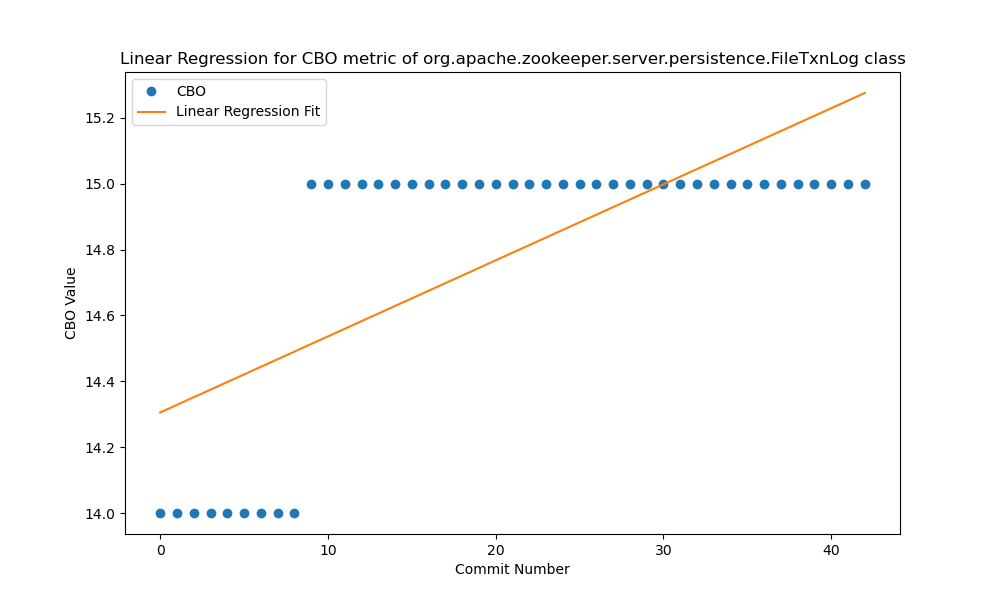
\includegraphics[width=0.8\linewidth]{figuras/343-83cf0a93c37759334fab885c2010fa0b7d953f52/Class-org.apache.zookeeper.server.persistence.FileTxnLog/CBO.png}
    \caption{CBO da classe \textit{org.apache.zookeeper.server.persistence.FileTxnLog}.}
    \label{fig:CBO3xPerformanceClass}
\end{figure}

\begin{figure}[h]
    \centering
    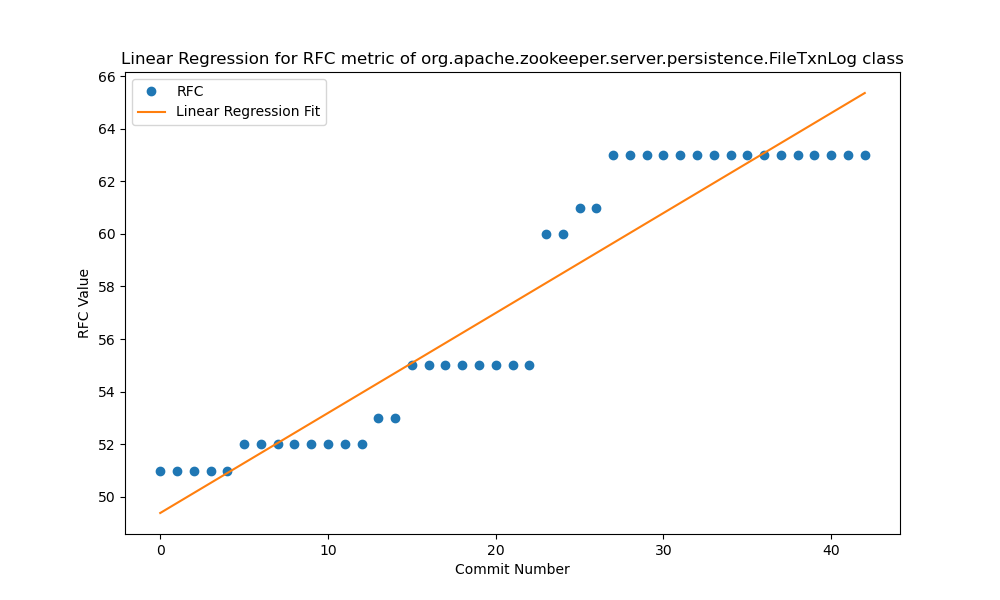
\includegraphics[width=0.8\linewidth]{figuras/343-83cf0a93c37759334fab885c2010fa0b7d953f52/Class-org.apache.zookeeper.server.persistence.FileTxnLog/RFC.png}
    \caption{RFC da classe \textit{org.apache.zookeeper.server.persistence.FileTxnLog}.}
    \label{fig:RFC3xPerformanceClass}
\end{figure}

\begin{figure}[h]
    \centering
    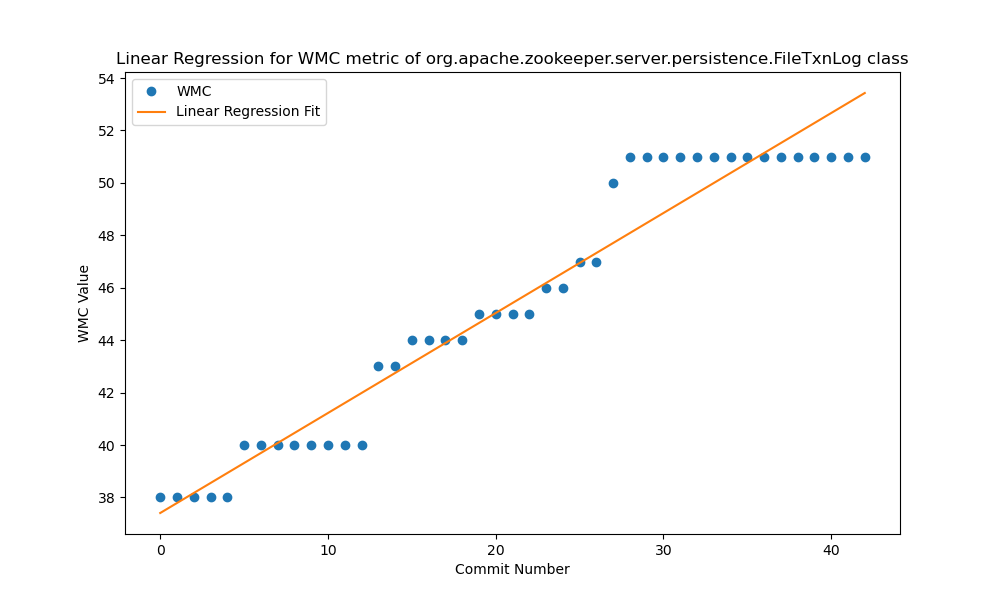
\includegraphics[width=0.8\linewidth]{figuras/343-83cf0a93c37759334fab885c2010fa0b7d953f52/Class-org.apache.zookeeper.server.persistence.FileTxnLog/WMC.png}
    \caption{WMC da classe \textit{org.apache.zookeeper.server.persistence.FileTxnLog}.}
    \label{fig:WMC3xPerformanceClass}
\end{figure}

A falta de uma refatoração mais substancial e a existência de uma melhoria de desempenho que não pôde ser validada tornam este \textit{commit} inadequado para servir como objeto de exemplo trabalhado. Além disso, uma vez que a classe \textit{``BufferedOutputStream''} está presente desde a versão inicial do Java (lançada em 1996) e o \textit{commit} em questão é de 2009, ou seja, o uso de um \textit{buffered input} devia ter sido feita desde o começo do projeto.

% Adicionar pelo menos mais um exemplo de commit analisado.

Observou-se que parte da complexidade na análise de um \textit{commit} propriamente dito reside na existência de uma considerável poluição nos dados. Muitos \textit{commits} no repositório do \textit{``ZooKeeper''} abrangem alterações em inúmeros arquivos, frequentemente incorporando refatorações não diretamente correlacionadas às mensagens de \textit{commit}. Essa complexidade aumenta a dificuldade de discernir as motivações subjacentes por trás das mudanças no código-fonte, tornando desafiador o processo de vincular essas alterações a possíveis vulnerabilidades identificadas externamente. Este fenômeno destaca a importância de uma abordagem criteriosa na interpretação do histórico de \textit{commits} para extrair conclusões significativas sobre a evolução do \textit{software} em relação à qualquer aspecto desejado.

\section{Heurística}
\label{sec:heuristica}

A heurística, ainda a ser concluída no TCC2, tem como finalidade auxiliar na criação de exemplos trabalhados para a \gls{es} por meio da análise da evolução do código nos repositórios selecionados, baseou-se em uma abordagem sistemática que envolve a escolha cuidadosa dos projetos, a seleção de métricas apropriadas e o desenvolvimento de ferramentas específicas para a análise. Primeiramente, foram estabelecidos critérios para a seleção de repositórios por meio de fatores como, ser um \gls{sds}, desenvolvido em Java, \textit{open-source}, ativamente mantido e utilizado em aplicações do mundo real. Os projetos escolhidos, \textit{Apache Kafka} e \textit{ZooKeeper}, destacaram-se por sua relevância no mercado de trabalho.

As métricas selecionadas inicialmente, como \gls{cbo}, \gls{rfc}, e \gls{wmc}, foram escolhidas para fornecer uma visão abrangente da qualidade do código, abordando diferentes aspectos. No entanto, durante o desenvolvimento do estudo, a métrica \gls{cbom} foi removida devido à percepção de que poderia introduzir poluição nos dados, comprometendo a integridade das métricas escolhidas.

Para a análise da evolução do código, foram desenvolvidas cinco ferramentas específicas, como \textit{code\_metrics.py}, \textit{metrics\_changes.py}, \textit{track\_files.py}, \textit{metrics\_evolution\_refactors.py}, e \textit{repository\_refactors.py.py}. Essas ferramentas foram implementadas em Python, utilizando o \textit{PyDriller} e o \textit{RefactoringMiner}, e estão disponíveis no Github \footnote{https://github.com/BrenoFariasdaSilva/Scientific-Research}.

Em síntese, a heurística inicialmente desenvolvida visa fornecer uma abordagem sistemática e contextualizada para a análise da evolução do código em \gls{sds}, reconhecendo as complexidades e desafios inerentes a essa tarefa, mas que, de fato, só será concluída no TCC2.

\section{Limitações}
\label{sec:limitacoes}

% Limitações do projeto de pesquisa.
Este trabalho apresenta uma limitação, a qual reside na impossibilidade de realizar análises empíricas de certas melhorias de desempenho, como a análise das trocas de mensagens em tempo real, devido à restrição ao uso de métricas estáticas de código. Isso impede a avaliação prática por meio da execução de \gls{sds} e simulações em grande escala, representando uma restrição na obtenção de percepções detalhadas sobre o desempenho em contextos de uma quantidade massiva de requisições sendo enviadas ao \gls{sd}. Além disso, poucos repositórios usam a conveção de \textit{commits}, o que facilitaria obter refatorações significativas, não poluídas por refatorações irrelevantes \cite{conventionalcommits}.

\chapter{Conclusões}
\label{chapter:conclusions}

O presente trabalho de pesquisa buscou investigar a evolução do código em \gls{sds} por meio da análise de métricas de código, com o intuito de criar exemplos trabalhados aplicáveis ao ensino de \gls{es}. A pesquisa foi orientada por quatro questões principais, delineando uma abordagem exploratória e qualitativa para compreender a relação entre métricas de código e melhorias em \gls{sds}, bem como para desenvolver exemplos trabalhados pedagogicamente eficazes para a \gls{es}.

Na formulação das questões de pesquisa, destacamos a importância de identificar métricas relevantes para analisar a evolução em \gls{sds}, observar padrões e tendências associados a melhorias no código, avaliar o impacto das métricas escolhidas em melhorias de desempenho, segurança, entre outros, e, finalmente, transformar essas melhorias em exemplos trabalhados para o ensino de \gls{es}.

A abordagem proposta fundamentou-se na compreensão da complexidade inerente aos \gls{sds} na era digital, justificando a necessidade de estudar a evolução do código para formar profissionais qualificados. A heurística desenvolvida para a seleção de códigos representativos de melhorias mostrou-se vital para delimitar o escopo de código a ser analisado, de modo a tentar criar exemplos trabalhados que ilustram, de forma prática, a dinâmica da evolução do código em \gls{sds}.

A escolha criteriosa das ferramentas, como CK, RefactoringMiner e PyDriller, permitiu uma análise abrangente das métricas de código e das mudanças ao longo do tempo nos repositórios selecionados. Destacamos a importância do Apache Kafka e ZooKeeper como repositórios relevantes, dada sua significativa presença em \gls{sds}, proporcionando um ambiente propício para a análise da evolução do código em \gls{sds}.

A metodologia adotada pretende possibilitar uma compreensão holística da relação entre métricas específicas e melhorias no código, indo além de uma abordagem quantitativa para incorporar elementos qualitativos na análise. A seleção de exemplos de código trabalhados baseados na heurística desenvolvida visa contribuir diretamente para o ensino de \gls{es}, fornecendo material prático e aplicável aos estudantes.

Os resultados prévios e o cronograma delinearam as fases da pesquisa, desde a revisão da literatura até a avaliação da utilidade educacional dos exemplos escolhidos. O cronograma ofereceu uma estrutura clara para as atividades planejadas ao longo dos meses, assegurando uma abordagem sistemática e eficiente na realização dos objetivos da pesquisa. Atualmente, nossos resultados destacam desafios, alguns dos quais eram esperados desde o início do projeto, relacionados à falta de padrão nos \textit{commits} e ao grande número de refatorações por \textit{commit}, muitas vezes não diretamente alinhadas à mensagem do \textit{commit}.

Em síntese, este trabalho visa preencher uma lacuna na literatura sobre a criação de exemplos trabalhados em \gls{es}, utilizando os \gls{sds} como objeto de estudo, contribuindo para a formação de estudantes e profissionais em \gls{es}. Ao proporcionar uma compreensão mais profunda da evolução do código em \gls{sds} e oferecer exemplos trabalhados pedagogicamente valiosos, espera-se impactar positivamente o ensino e a prática profissional na área de \gls{es}.


%% Formatação de páginas de elementos pós-textuais
\postextual%% Não comente esta linha

%% Arquivos de referências
\arquivosdereferencias{%% Arquivos bibtex sem a extensão .bib e separados por vírgula - Não comente esta linha
  %./PosTexto/exemplos-referencias,%% Arquivo de referências - Comente para remover este item
  main%% Arquivo de referências - Comente para remover este item
}%% Não comente esta linha

%% Glossário
%\incluirglossario %% Comente para remover este item

%% Arquivos de apêndices
 %\begin{arquivosdeapendices}%% Os arquivos de apêndices devem se incluídos neste ambiente - Não comente esta linha
%   %\partapendices%% Página de início dos apêndices - adiciona uma página com o título Apêndices
%   %% Capítulo de exemplo
   %%%%% APÊNDICE A
%%
%% Texto ou documento elaborado pelo autor, a fim de complementar sua argumentação, sem prejuízo da unidade nuclear do trabalho.

%% Título e rótulo de apêndice (rótulos não devem conter caracteres especiais, acentuados ou cedilha)
\chapter{Título do Apêndice A com um Texto Muito Longo que Pode Ocupar Mais de uma Linha}\label{cap:apendicea}

Quando houver necessidade pode-se apresentar como apêndice documento(s) auxiliar(es) e/ou complementar(es) como: legislação, estatutos, gráficos, tabelas, etc. Os apêndices são enumerados com letras maiúsculas: \autoref{cap:apendicea}, \autoref{cap:apendiceb}, etc.

No \latex\ apêndices são editados como capítulos. O comando \verb|\appendix| faz com que todos os capítulos seguintes sejam considerados apêndices.

Apêndices complementam o texto principal da tese com informações para leitores com especial interesse no tema, devendo ser considerados leitura opcional, ou seja, o entendimento do texto principal da tese não deve exigir a leitura atenta dos apêndices.

Apêndices usualmente contemplam provas de teoremas, deduções de fórmulas matemáticas, diagramas esquemáticos, gráficos e trechos de código. Quanto a este último, código extenso não deve fazer parte da tese, mesmo como apêndice. O ideal é disponibilizar o código na Internet para os interessados em examiná-lo ou utilizá-lo.

%% Título e rótulo de seção (rótulos não devem conter caracteres especiais, acentuados ou cedilha)
%\section{Título da Seção Secundária do Apêndice B}\label{sec:secaoapendicea}

%Exemplo de seção secundária em apêndice (\autoref{sec:secaoapendicea} do \autoref{cap:apendicea}).

%% Título e rótulo de seção (rótulos não devem conter caracteres especiais, acentuados ou cedilha)
%\subsection{Título da Seção Terciária do Apêndice B}\label{subsec:subsecaoapendicea}

%Exemplo de seção terciária em apêndice (\autoref{subsec:subsecaoapendicea} do \autoref{cap:apendicea}).

%% Título e rótulo de seção (rótulos não devem conter caracteres especiais, acentuados ou cedilha)
%\subsubsection{Título da seção quaternária do Apêndice B}\label{subsubsec:subsubsecaoapendicea}

%Exemplo de seção quaternária em apêndice (\autoref{subsubsec:subsubsecaoapendicea} do \autoref{cap:apendicea}).

%% Título e rótulo de seção (rótulos não devem conter caracteres especiais, acentuados ou cedilha)
%\paragraph{Título da seção quinária do Apêndice B}\label{para:paragraphapendicea}

%Exemplo de seção quinária em apêndice (\autoref{para:paragraphapendicea} do \autoref{cap:apendicea}).
%% Apêndice - Comente para remover este item
   %%%%% APÊNDICE B
%%
%% Texto ou documento elaborado pelo autor, a fim de complementar sua argumentação, sem prejuízo da unidade nuclear do trabalho.

%% Título e rótulo de apêndice (rótulos não devem conter caracteres especiais, acentuados ou cedilha)
\chapter{Orçamentos dos Materiais para Montagem da Bancada Experimental}\label{cap:apendiceb}

\begin{table}[htb]%% Ambiente table
\caption{Orçamento dos materiais n.\textsuperscript{o} 1.}%% Legenda
\label{tab:tab3}%% Rótulo
\begin{tabularx}{\textwidth}{@{\extracolsep{\fill}}lrrr}%% Ambiente tabularx
\toprule
Material              & \multicolumn{1}{c}{Valor (R\$)} & \multicolumn{1}{c}{Quantidade}  & \multicolumn{1}{c}{Total (R\$)} \\ \midrule
Bomba centrífuga      & 2500,00                         & 01                              & 2500,00                         \\
Compressor rotativo   & 3000,00                         & 01                              & 3000,00                         \\
Manômetro diferencial & 450,00                          & 02                              & 900,00                          \\
Termopar              & 370,00                          & 02                              & 740,00                          \\
Válvula de esfera     & 43,00                           & 02                              & 86,00                           \\
Tubulação de PVC      & 10,00                           & 05                              & 50,00                           \\
Conexão de PVC        & 5,00                            & 10                              & 50,00                           \\ \midrule
                      &                                 & \multicolumn{1}{r}{Total (R\$)} & 7326,00                         \\ \bottomrule
\end{tabularx}
\fonte{}%% Fonte
\end{table}

\begin{table}[htb]%% Ambiente table
\caption{Orçamento dos materiais n.\textsuperscript{o} 2.}%% Legenda
\label{tab:tab4}%% Rótulo
\begin{tabularx}{\textwidth}{@{\extracolsep{\fill}}lrrr}%% Ambiente tabularx
\toprule
Material              & \multicolumn{1}{c}{Valor (R\$)} & \multicolumn{1}{c}{Quantidade}  & \multicolumn{1}{c}{Total (R\$)} \\ \midrule
Bomba centrífuga      & 2700,00                         & 01                              & 2700,00                         \\
Compressor rotativo   & 2950,00                         & 01                              & 2950,00                         \\
Manômetro diferencial & 515,00                          & 02                              & 1030,00                         \\
Termopar              & 350,00                          & 02                              & 700,00                          \\
Válvula de esfera     & 40,00                           & 02                              & 80,00                           \\
Tubulação de PVC      & 8,00                            & 05                              & 40,00                           \\
Conexão de PVC        & 6,00                            & 10                              & 60,00                           \\ \midrule
                      &                                 & \multicolumn{1}{r}{Total (R\$)} & 7560,00                         \\ \bottomrule
\end{tabularx}
\fonte{}%% Fonte
\end{table}

\begin{table}[htb]%% Ambiente table
\caption{Orçamento dos materiais n.\textsuperscript{o} 3.}%% Legenda
\label{tab:tab5}%% Rótulo
\begin{tabularx}{\textwidth}{@{\extracolsep{\fill}}lrrr}%% Ambiente tabularx
\toprule
Material              & \multicolumn{1}{c}{Valor (R\$)} & \multicolumn{1}{c}{Quantidade}  & \multicolumn{1}{c}{Total (R\$)} \\ \midrule
Bomba centrífuga      & 2600,00                         & 01                              & 2600,00                         \\
Compressor rotativo   & 3100,00                         & 01                              & 3100,00                         \\
Manômetro diferencial & 500,00                          & 02                              & 1000,00                         \\
Termopar              & 400,00                          & 02                              & 800,00                          \\
Válvula de esfera     & 45,00                           & 02                              & 90,00                           \\
Tubulação de PVC      & 12,00                           & 05                              & 60,00                           \\
Conexão de PVC        & 5,00                            & 10                              & 50,00                           \\ \midrule
                      &                                 & \multicolumn{1}{r}{Total (R\$)} & 7700,00                         \\ \bottomrule
\end{tabularx}
\fonte{}%% Fonte
\end{table}
%% Apêndice - Comente para remover este item
 %\end{arquivosdeapendices}%% Não comente esta linha


% \begin{apendicesenv}%% Ambiente apendicesenv

% \partapendices
% \chapter{Ola}

% \lipsum[55-56]

% \end{apendicesenv}

%% Arquivos de anexos
%\begin{arquivosdeanexos}%% Os arquivos de anexos devem se incluídos neste ambiente - Não comente esta linha
  %\partanexos%% Página de início dos anexos - adiciona uma página com o título Anexos

  % %%%% ANEXO A
%%
%% Texto ou documento não elaborado pelo autor, que serve de fundamentação, comprovação e ilustração.

%% Título e rótulo de anexo (rótulos não devem conter caracteres especiais, acentuados ou cedilha)
\anexos
\chapter{Direitos Autorais - Lei N\texorpdfstring{.\textsuperscript{o}}{o.} 9.610, de 19 de Fevereiro de 1998: Disposições Preliminares}\label{cap:anexoa}

\centerline{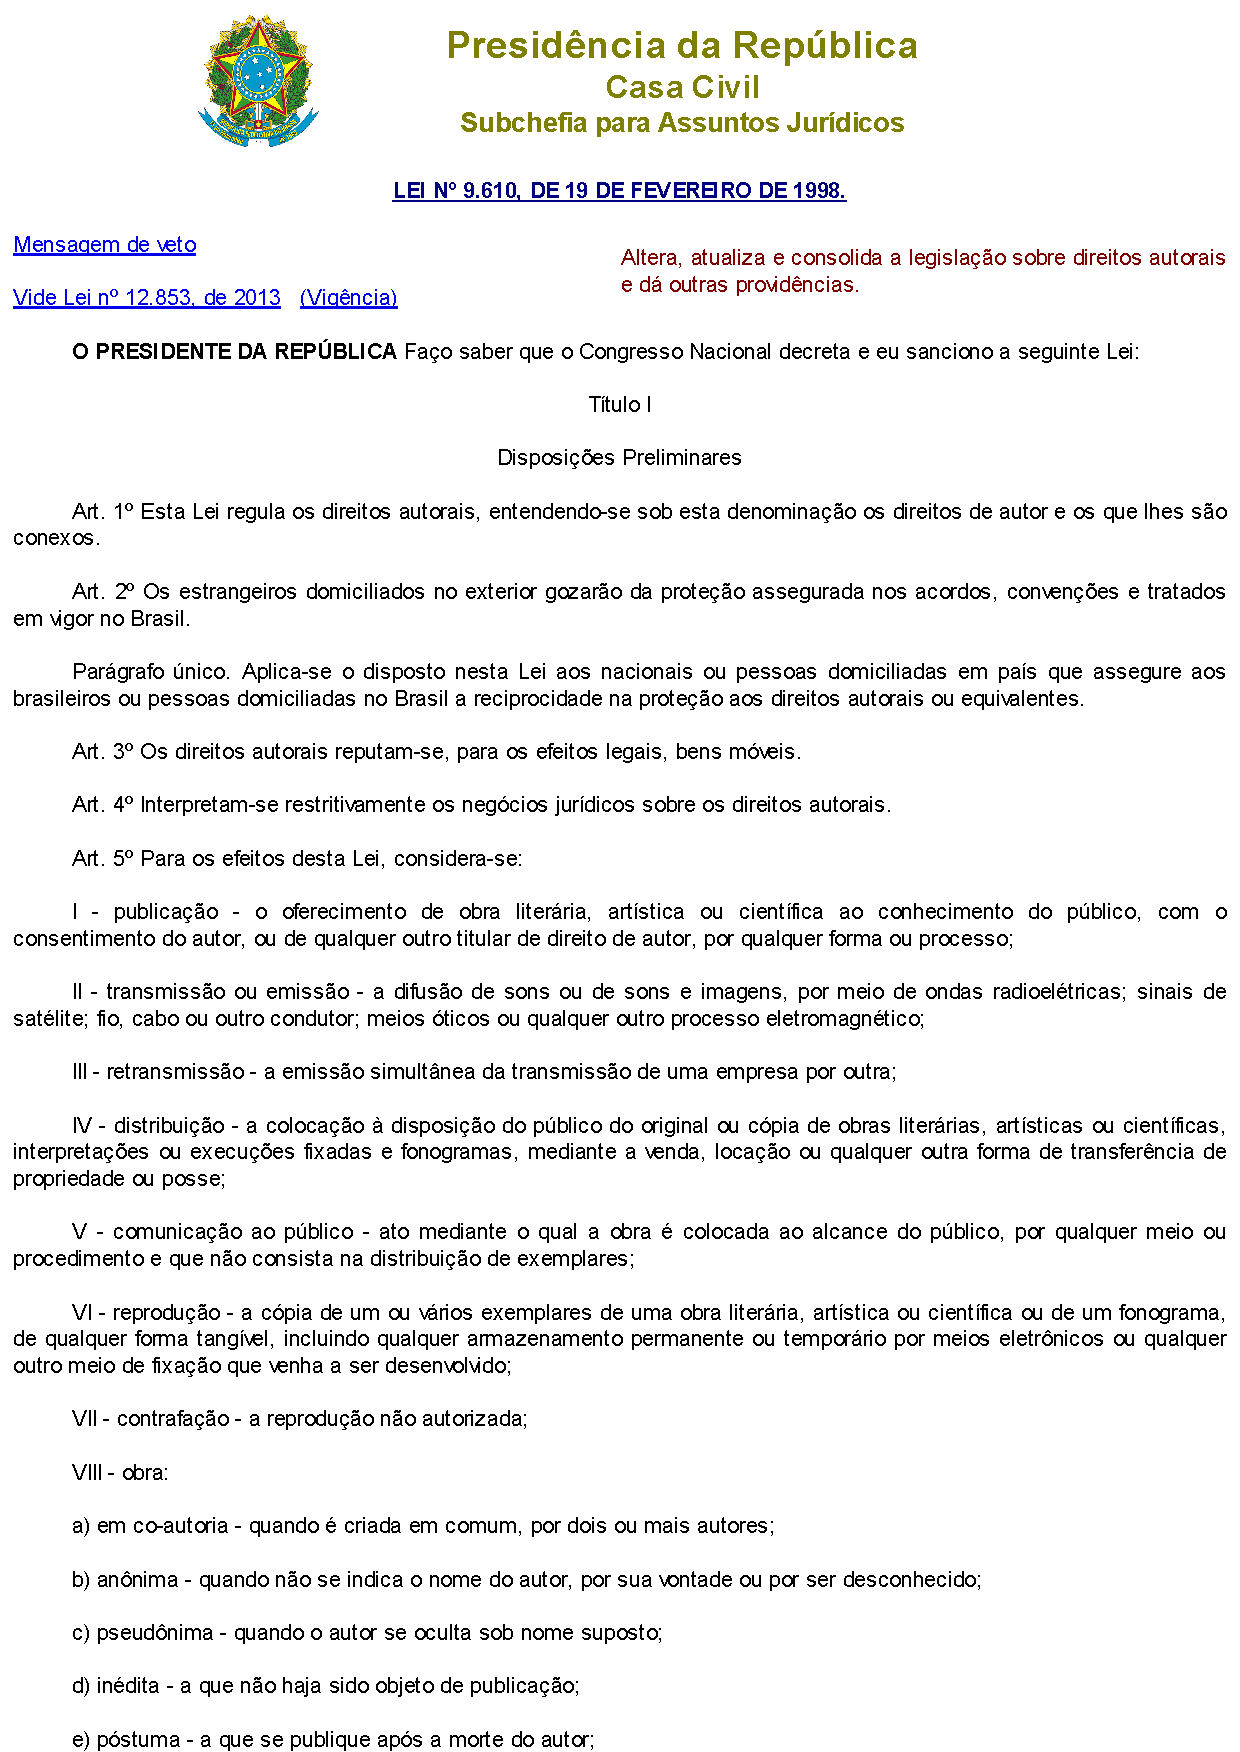
\includegraphics[width=\textwidth]{./PosTexto/Ilustracoes/lei-n9610-p1}}%% Imagem (Dimensões e localização)

\centerline{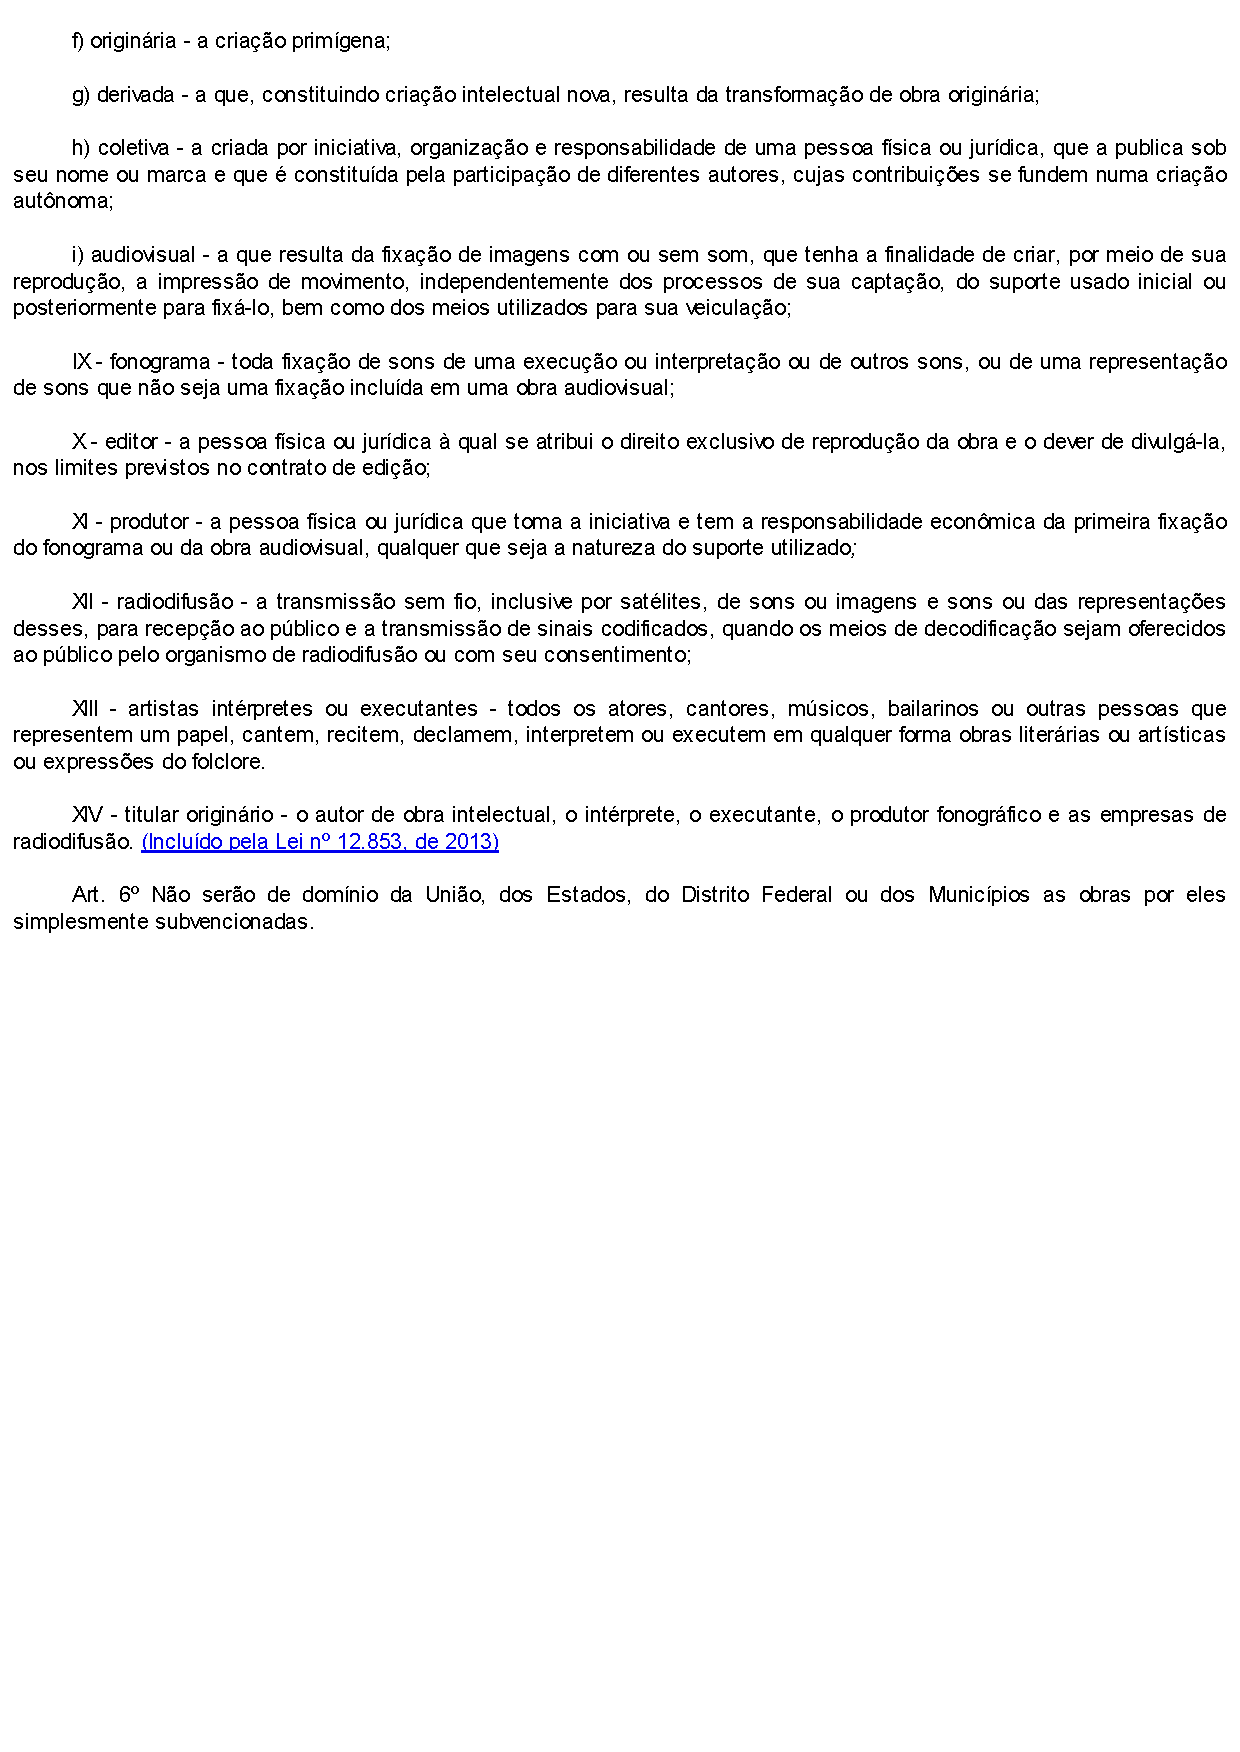
\includegraphics[width=\textwidth]{./PosTexto/Ilustracoes/lei-n9610-p2}}%% Imagem (Dimensões e localização)
%% Anexo - Comente para remover este item
  % %%%% ANEXO B
%%
%% Texto ou documento não elaborado pelo autor, que serve de fundamentação, comprovação e ilustração.

%% Título e rótulo de anexo (rótulos não devem conter caracteres especiais, acentuados ou cedilha)
\chapter{Normas para Elaboração de Trabalhos Acadêmicos}\label{cap:anexob}

As normas da \gls{utfpr} podem ser acessadas em: \url{http://portal.utfpr.edu.br/biblioteca/trabalhos-academicos/discentes/orientacao-para-trabalhos-academicos}. Ver Figura \ref{fig:capadolivro}.

\begin{figure}[htb]%% Ambiente figure
\captionsetup{width=0.9\textwidth}%% Largura da legenda
\caption{Sítio: Normas para Elaboração de Trabalhos Acadêmicos.}%% Legenda
\label{fig:capadolivro}%% Rótulo
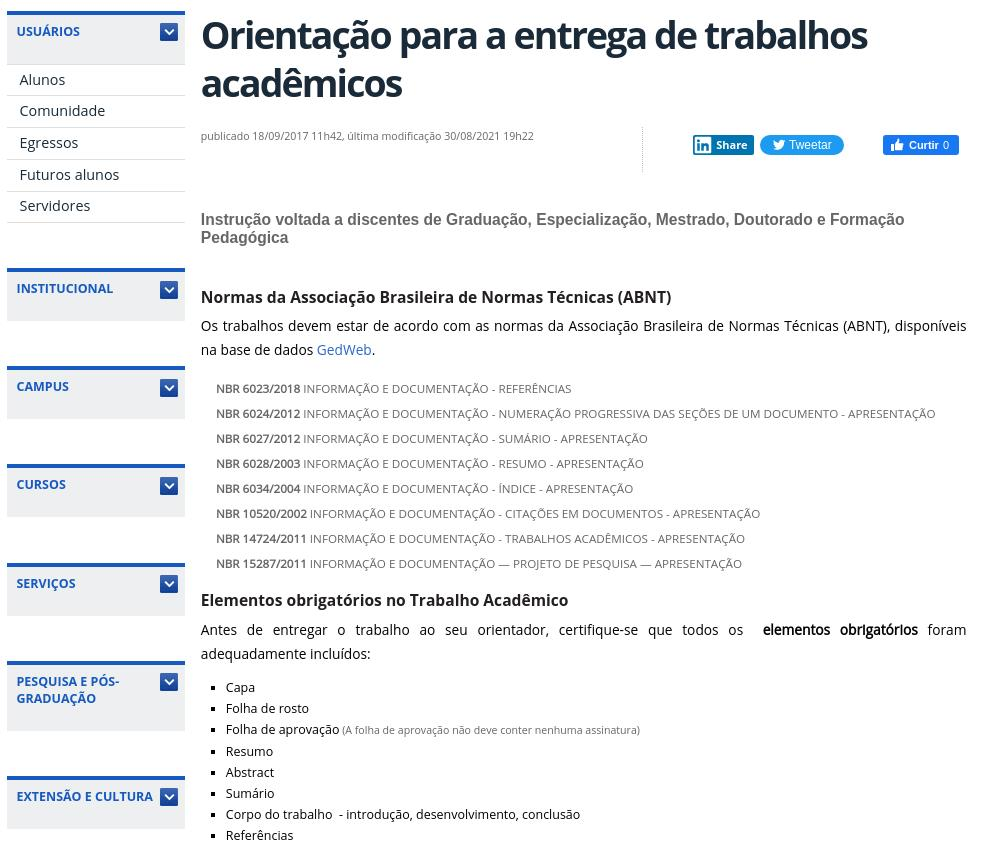
\includegraphics[width=0.9\textwidth]{normas}%% Dimensões e localização
\fonte{\cite{UTFPR2008}}%% Fonte
\end{figure}

%% Anexo - Comente para remover este item
%\end{arquivosdeanexos}%% Não comente esta linha

%% Índice - Adiciona um índice remissivo.
%\incluirindice%% Comente para remover este item

%% Fim do documento
\end{document}%% Não comente esta linha
